\newpage
\chapter{Design Changes}
\label{chap:design_changes}
% what major design changes have been introduced since the CDR report? Argument why these changes were necessary. Also, will be good to include test results (functionality, weight, performance etc.) which are not documented in the CDR report.
%
%
\section{Project Schedule, Resources and Goals}
\label{sec:project_changes}
%responsible: Morten
%
As previously stated in [CDR ref], the U-SPACE project was initially substantially delayed due to bureaucratic challenges in course registrations and subsequent release of project budget. This resulted in a reformulation of the system concept going from a custom designed helium envelope to a \ac{COTS} blimp provided by Esrange Space Center.

In June 2012, many of the U-SPACE team members left Kiruna to pursue summer internships and prepare for their 3rd semester outside Sweden. Work on the project over the summer holiday was restricted since Lars Jakobsson (LTU technician) was unavailable thus making ordering of new components impossible. Work on U-SPACE began again in September 2012, when Jan and Pedro returned to Sweden and Omair officially joined the project. At this point, Morten took over the full project management responsibilities and also remained responsible for the power subsystem, Jan became the lead responsible for the attitude sensors and payload, Omair responsible for all on-board telemetry handling, telecommunication and ground station and Pedro responsible for the mechanical structure and motors.

Since the sun sits very low on the horizon during autumn in Kiruna and is almost completely absent during winter, it was decided, for the first prototype, not to implement the solar array and related electronics. Instead the goal would be to realize an indoor battery powered flight. This also reduced the work load as was required due to the fewer people now working on the project.

Weekly status meetings were held with project supervisors, but internal meetings were only held on a need-basis since the group just counted four people and were often already sitting together in the Viking project room. 
Due to some misunderstandings of the initial budget, it was approved by the supervisors to increase the project budget for the four remaining students from 2000 SEK to 2500 SEK per student. 


\section{Electrical Power Subsystem}
%responsible: Morten
%
Due to the issues discussed in section \ref{sec:project_changes}, the solar cells were not ordered. However, it is still believed that the cells discussed in [ref to CDR] are suitable for this project.
%
%
In the final circuity layouts, it was decided to place the \ac{BCR} and \ac{SAR} on separate \acp{PCB}. Additionally, a small temperature sensor board was built. The following sections describe the features and circuit diagrams of each of these boards.
%
%
\subsection{Battery}
%
%Challenges in thermal design to achieve specifications on battery. A passive design has been made. Specify test results. Suggestion to add a heater or have a winter + summer configuration of the insulation.
%
During testing of a thermal design, one Li-ion battery underwent a heavy discharge and subsequently showed clear indication of damage (swallowing of the battery pack). There was no immediate danger, however the incidence learned us that it is important that everyone working with Li-ion batteries knows about its safe use and limitations. Li-ion fires are almost impossible to put out. Only useful method is to cover the battery in sand why we recommend LTU to put available a bucket of sand and/or establish a fire proof area/table for working with Li-ion batteries.
%
%
\subsection{Battery Charge Regulator}
%
Table \ref{tab:BCR_features} lists the features of the final \ac{BCR}.
%
\begin{table}[H]
\centering
\caption{Features of developed \ac{BCR}}
\label{tab:BCR_features}
\begin{tabular}{p{0.35\textwidth}p{0.2\textwidth}p{0.4\textwidth}}
\hline
\textbf{Feature/Specification} & \textbf{Value} & \textbf{Comments}\\
\hline
Max output current & 20 A & All outputs combined \\
Output voltage & 6-8 V & Unregulated \\
Input voltage & 9.2-9.5 V & Higher voltage may lead to overheating\\
Weight & ??? & \\
Under voltage protection & $V_{BATT}$ < 6.0 V & Only cuts off motor power outputs \\
Short-circuit protection & $I_{SC}$ > 15 A & Only on motor power outputs \\
Thermal monitoring and charge cut-off & & \\
Automatic charge control & - & Constant current or voltage and trickle charge\\
Charge inhibit by telecommand & & \\
Power cut-off by telecommand & & Only motor power outputs\\
Charge status telemetry & &\\
Charge/discharge current monitoring & & \\
Battery cells voltage monitoring & & \\
\hline
\end{tabular}
\end{table} 
%
The main changes to the \ac{BCR} include added telemetries, telecommands and protection circuits.
%
%
\subsubsection*{Increasing BCR Power Output}
The chosen Li-ion battery can supply up to 66 A continuously or 88 A burst. The main limitation of the \ac{BCR} power output is due to current ratings on the power diode (20 A), power connectors (19 A) and wires (19 A or 11.5 A when using ECSS derating[ref to ECSS]). PCB trace thickness may also become impractically thick at higher currents. 
To increase the output power rating, the best and first option is to use a higher battery voltage by connecting several batteries in series (or using a higher voltage battery pack with more cells in series). 
The current rating can also be increased by using higher power connectors, thicker wire or several wires in parallel, higher power diodes or two diodes in parallel and using thicker PCB copper tracing, reducing trace length, increasing trace width and improving the thermal layout (adding lots of heat sinks and thermal connections).
%
%
All \ac{BCR} functionalities have been tested and verified at room temperature conditions.
%
\begin{figure}[H]
\begin{minipage}[t]{\linewidth}
\centering
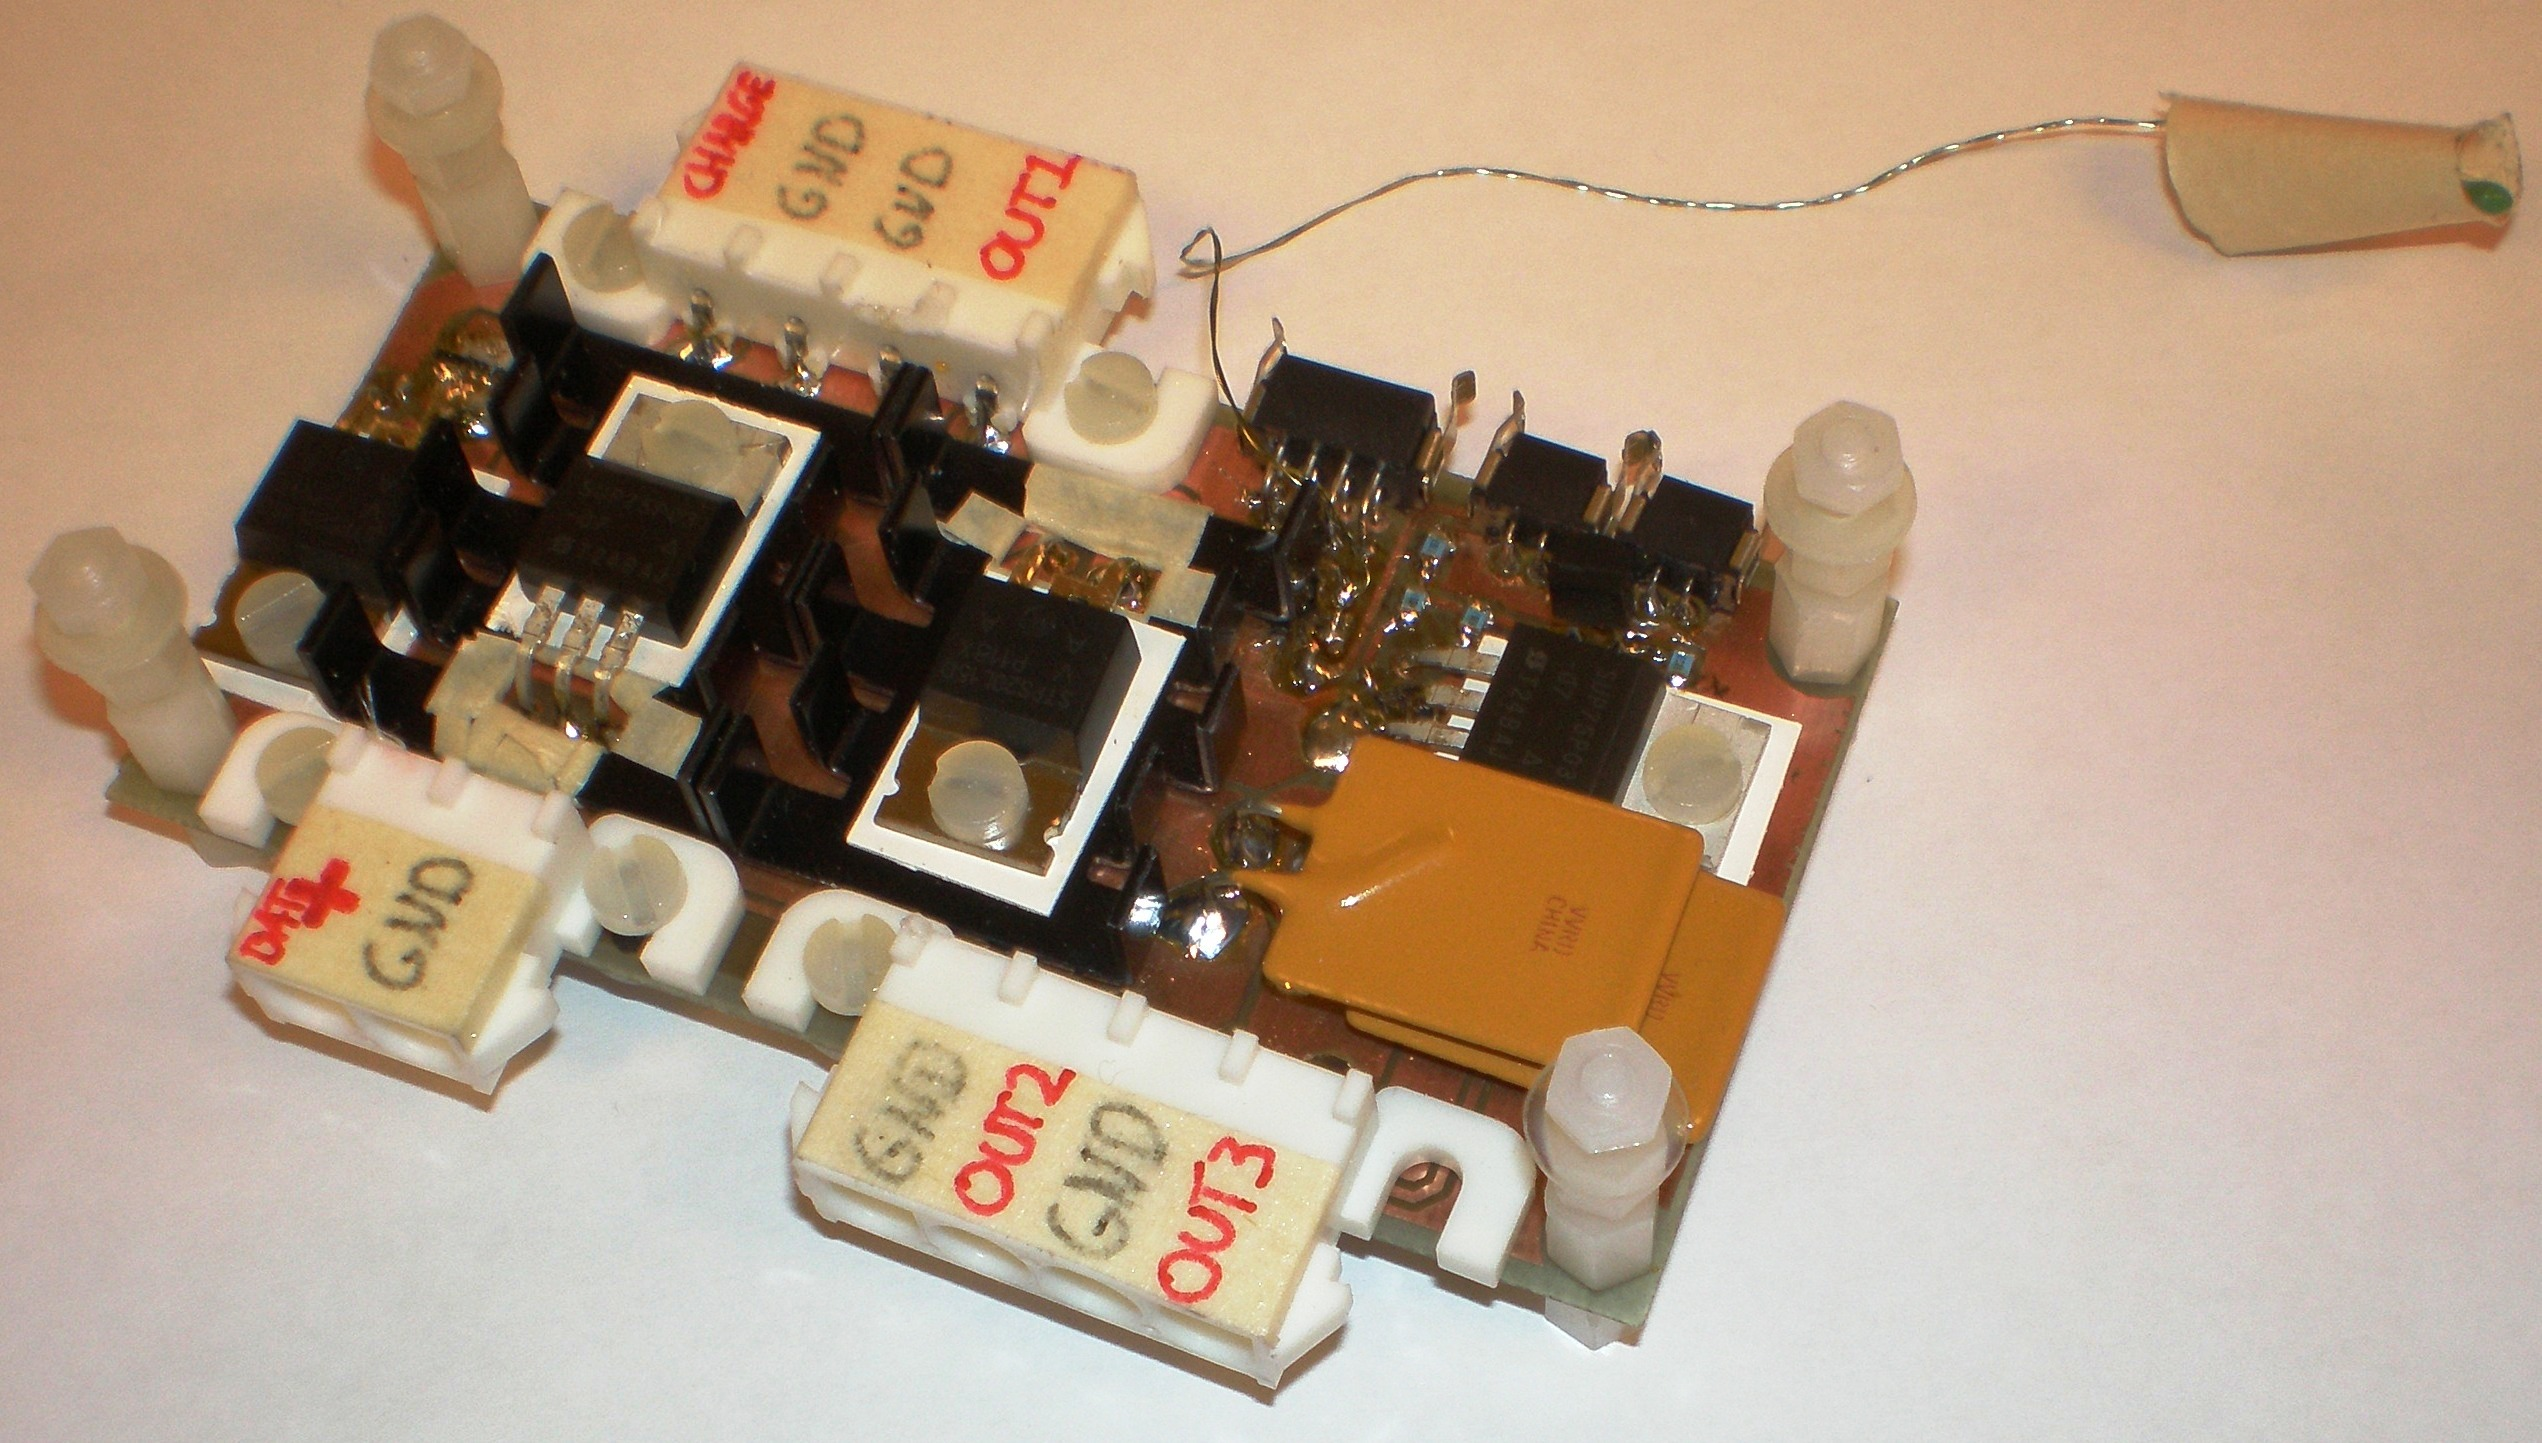
\includegraphics[width=0.7\textwidth]{figures/fig_BCR_top}
\end{minipage}
\vspace{2mm}
\begin{minipage}[t]{\linewidth}
\centering
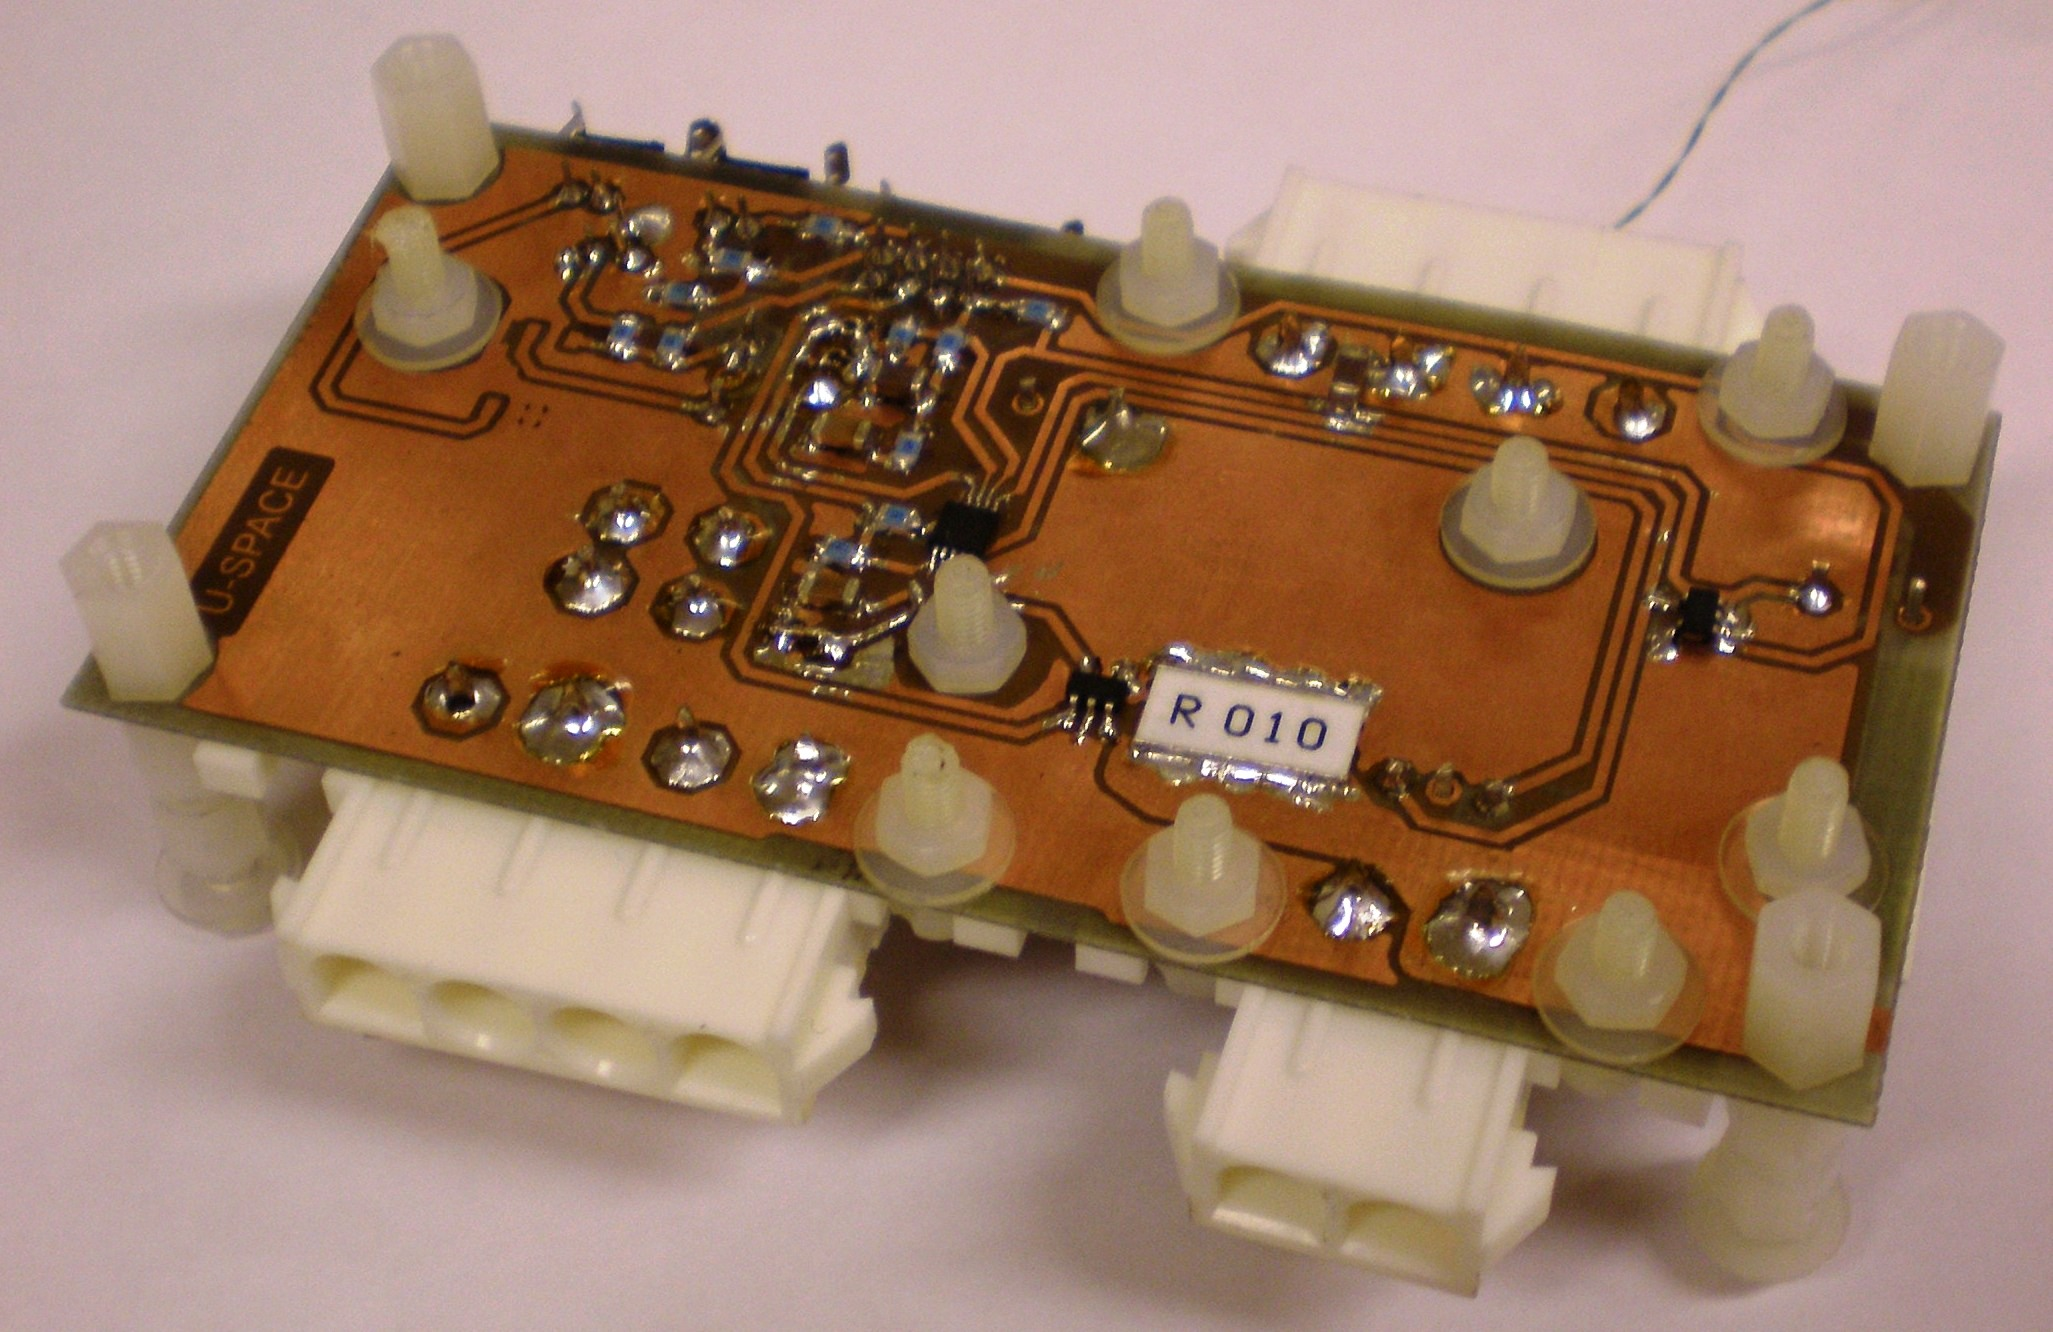
\includegraphics[width=0.7\textwidth]{figures/fig_BCR_bottom}
\end{minipage}
\caption{Battery Charge Regulator}
\label{fig:BCR_top_bottom}
\end{figure}
%
\begin{figure}[H]
\centering
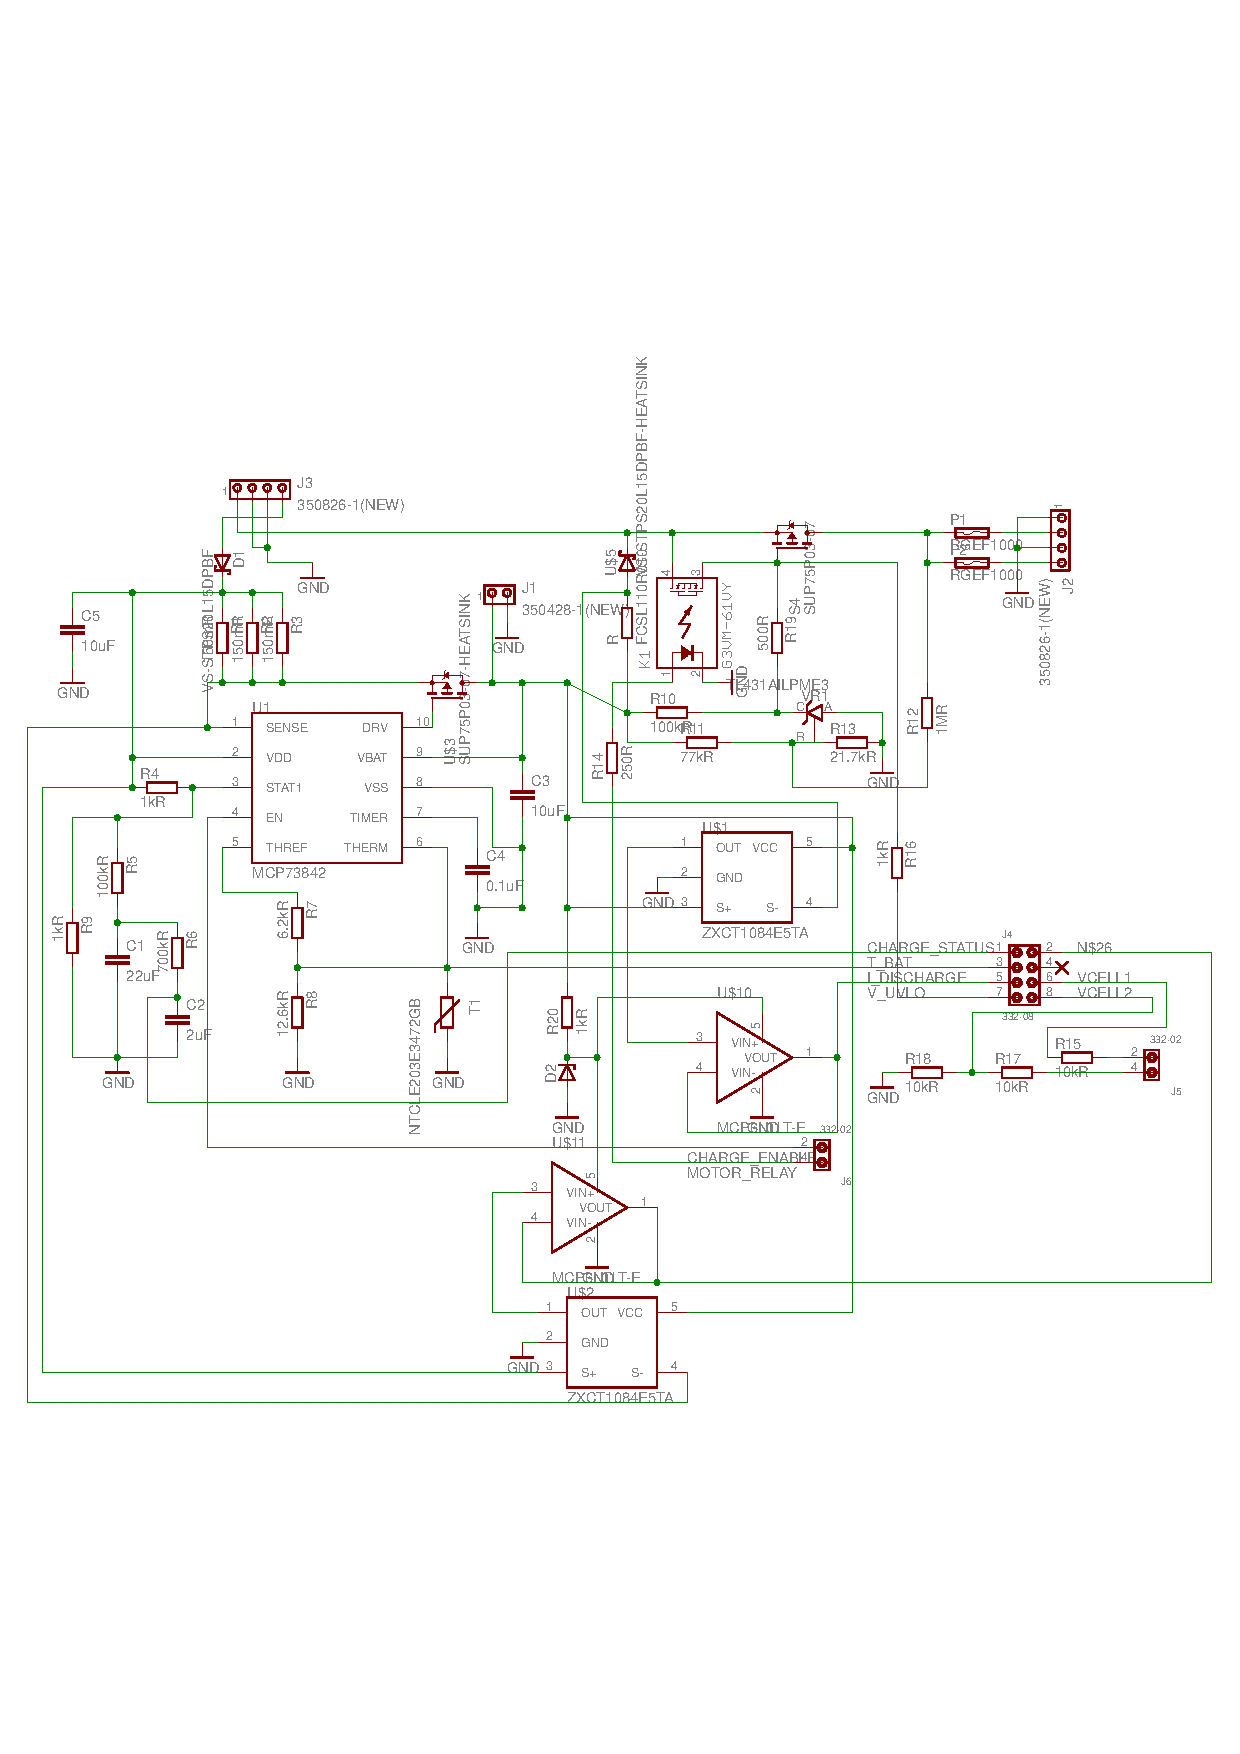
\includegraphics[width=\textwidth]{figures/fig_Schematic_BCR}
\caption{Schematic of the \acl{BCR}}
\label{fig:BCR_Schematic}
\end{figure}
%
%
\subsection{Solar Array Regulator}

5.0V(regulated), 3.3V(regulated),

Inclusion of 3.3V regulated output - mainly due to limitations on BeagleBoard which is not compatible with 5V?

SAR not implemented due to time limitation.

MPPT not implemented due to time limitation.

Components for DC-DC converter already ordered.

Additional telemetry data outputs added for SAR.

\begin{figure}[H]
\begin{minipage}[t]{\linewidth}
\centering
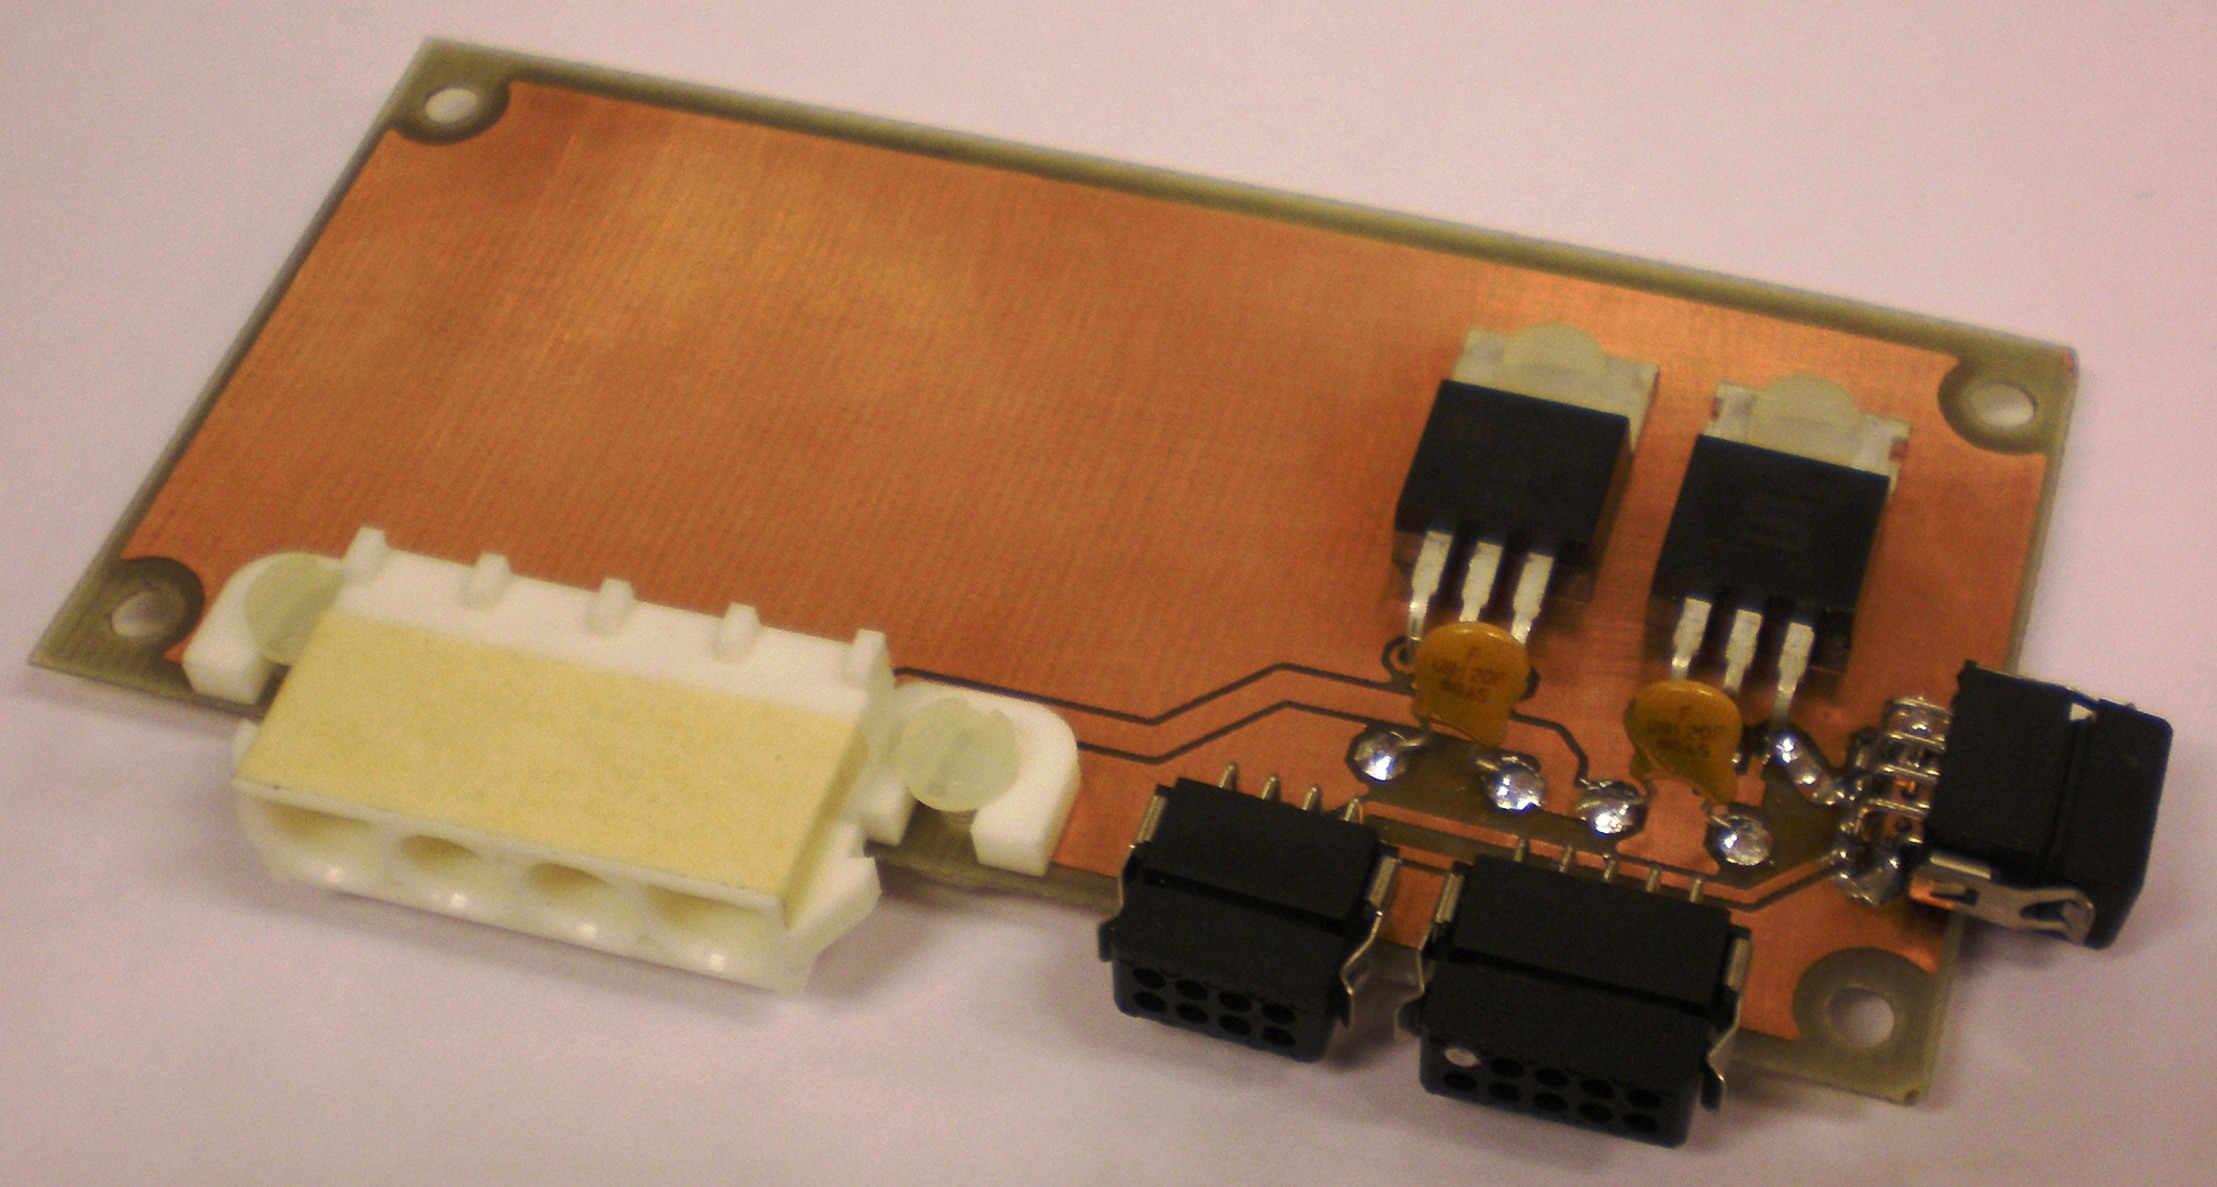
\includegraphics[width=0.7\textwidth]{figures/fig_SAR_top}
\end{minipage}
\vspace{2mm}
\begin{minipage}[t]{\linewidth}
\centering
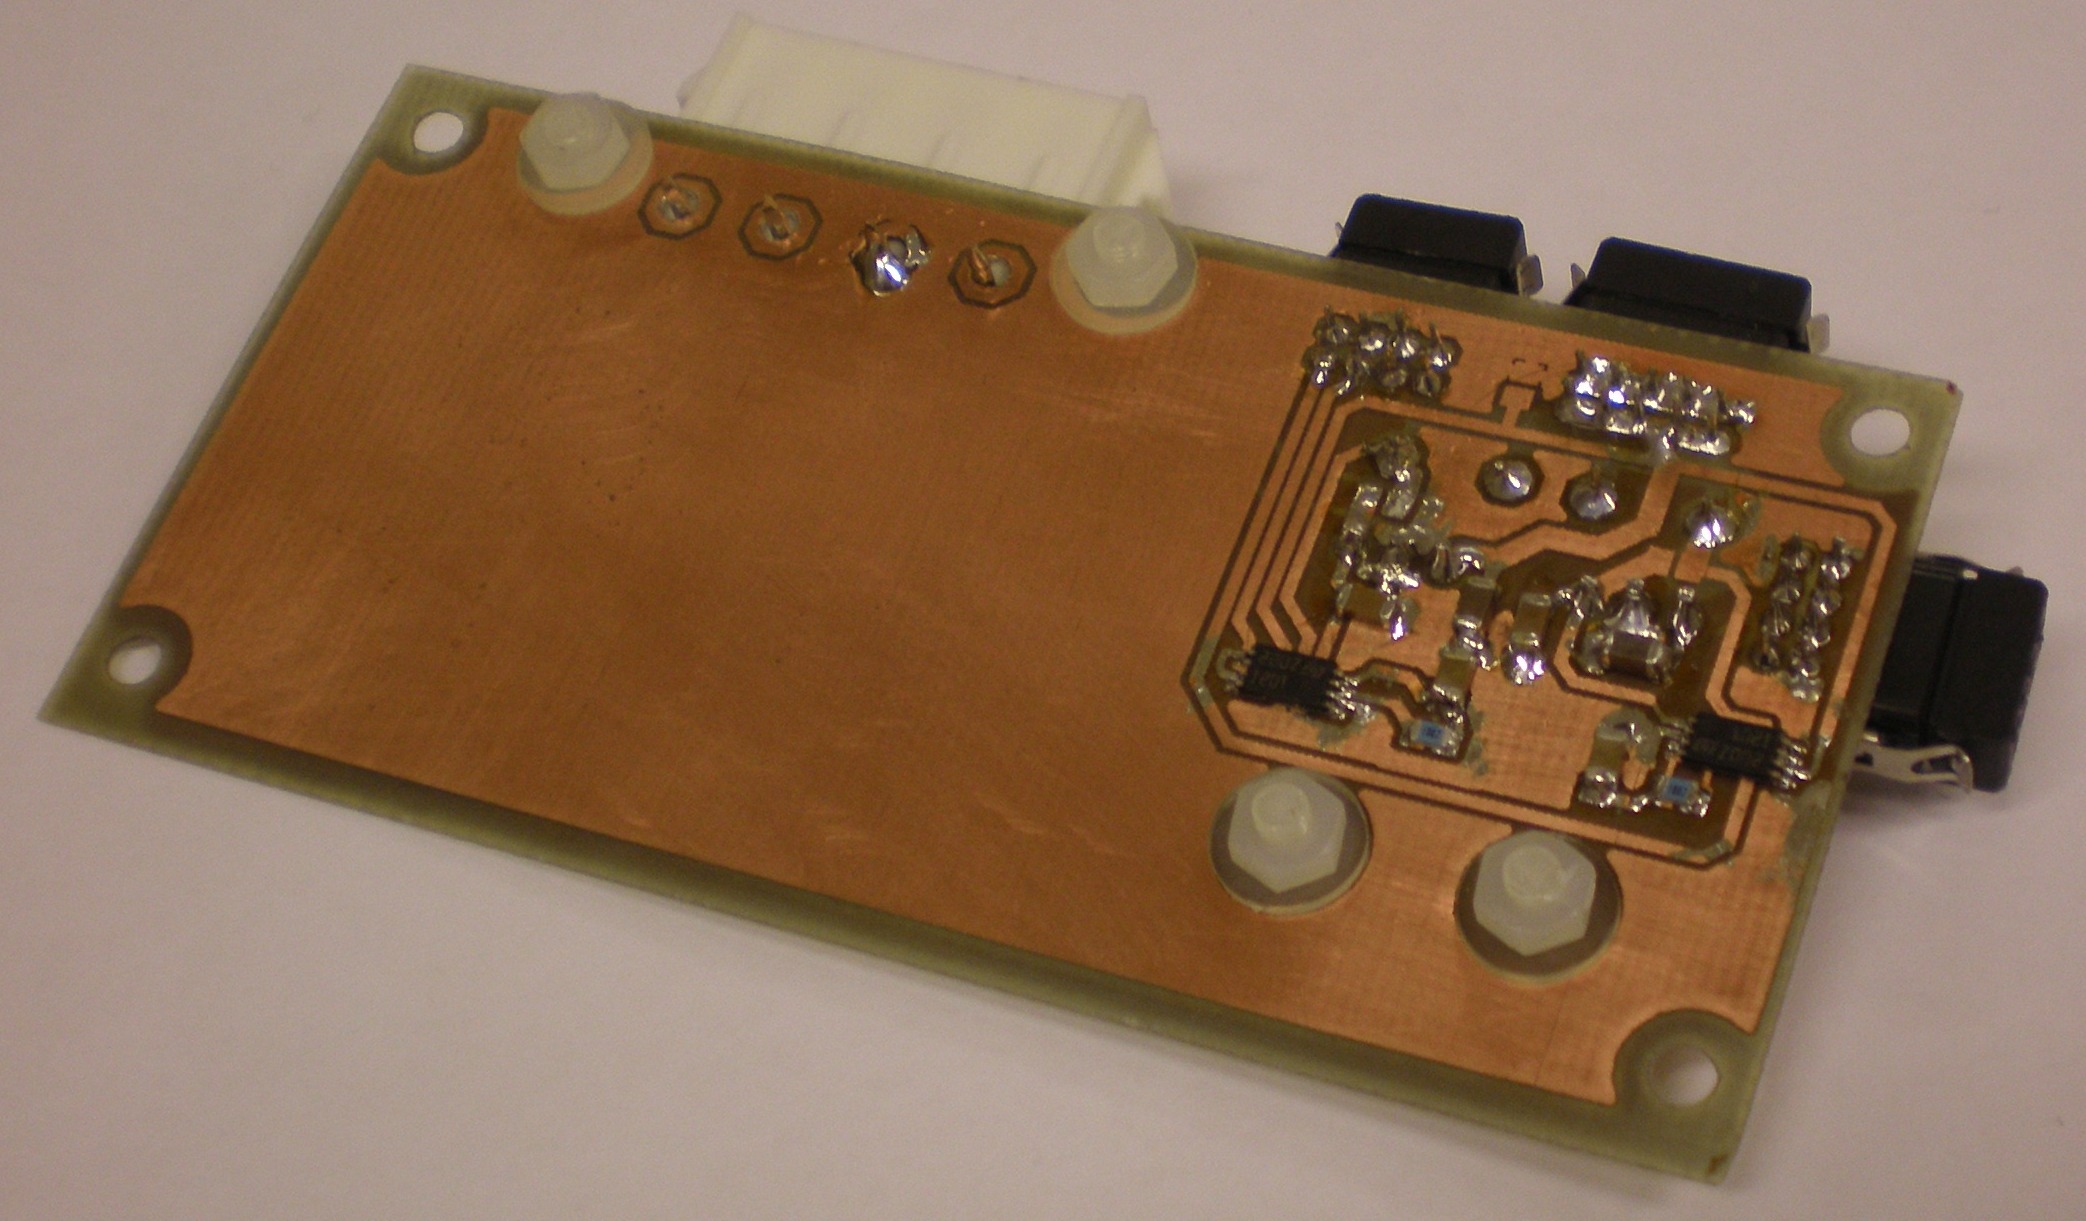
\includegraphics[width=0.7\textwidth]{figures/fig_SAR_bottom}
\end{minipage}
\caption{Battery Charge Regulator}
\label{fig:SAR_top_bottom}
\end{figure}

\begin{figure}[H]
\centering
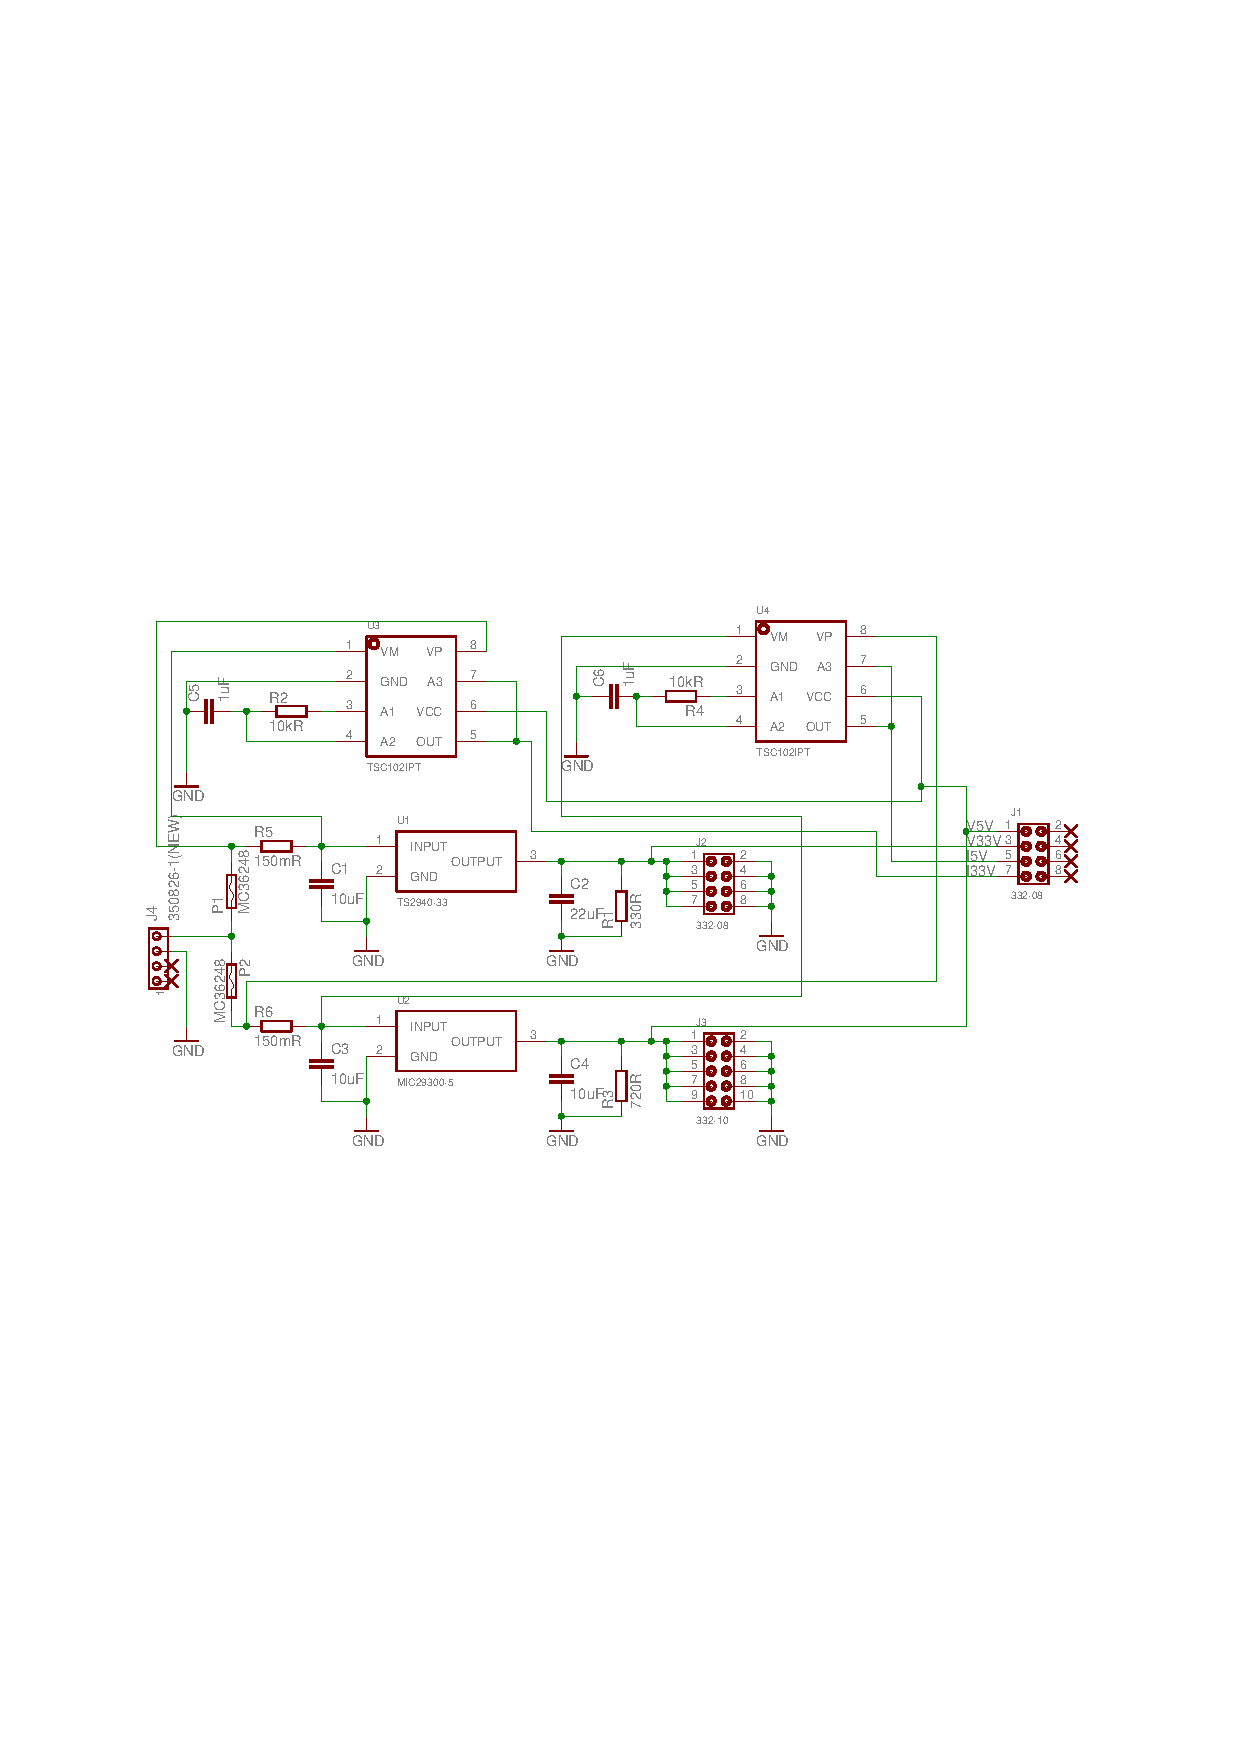
\includegraphics[width=\textwidth]{figures/fig_Schematic_SAR}
\caption{Schematic of the \acl{SAR}}
\label{fig:SAR_Schematic}
\end{figure}


\subsection{Temperature Sensor Board}


\begin{figure}[H]
\centering
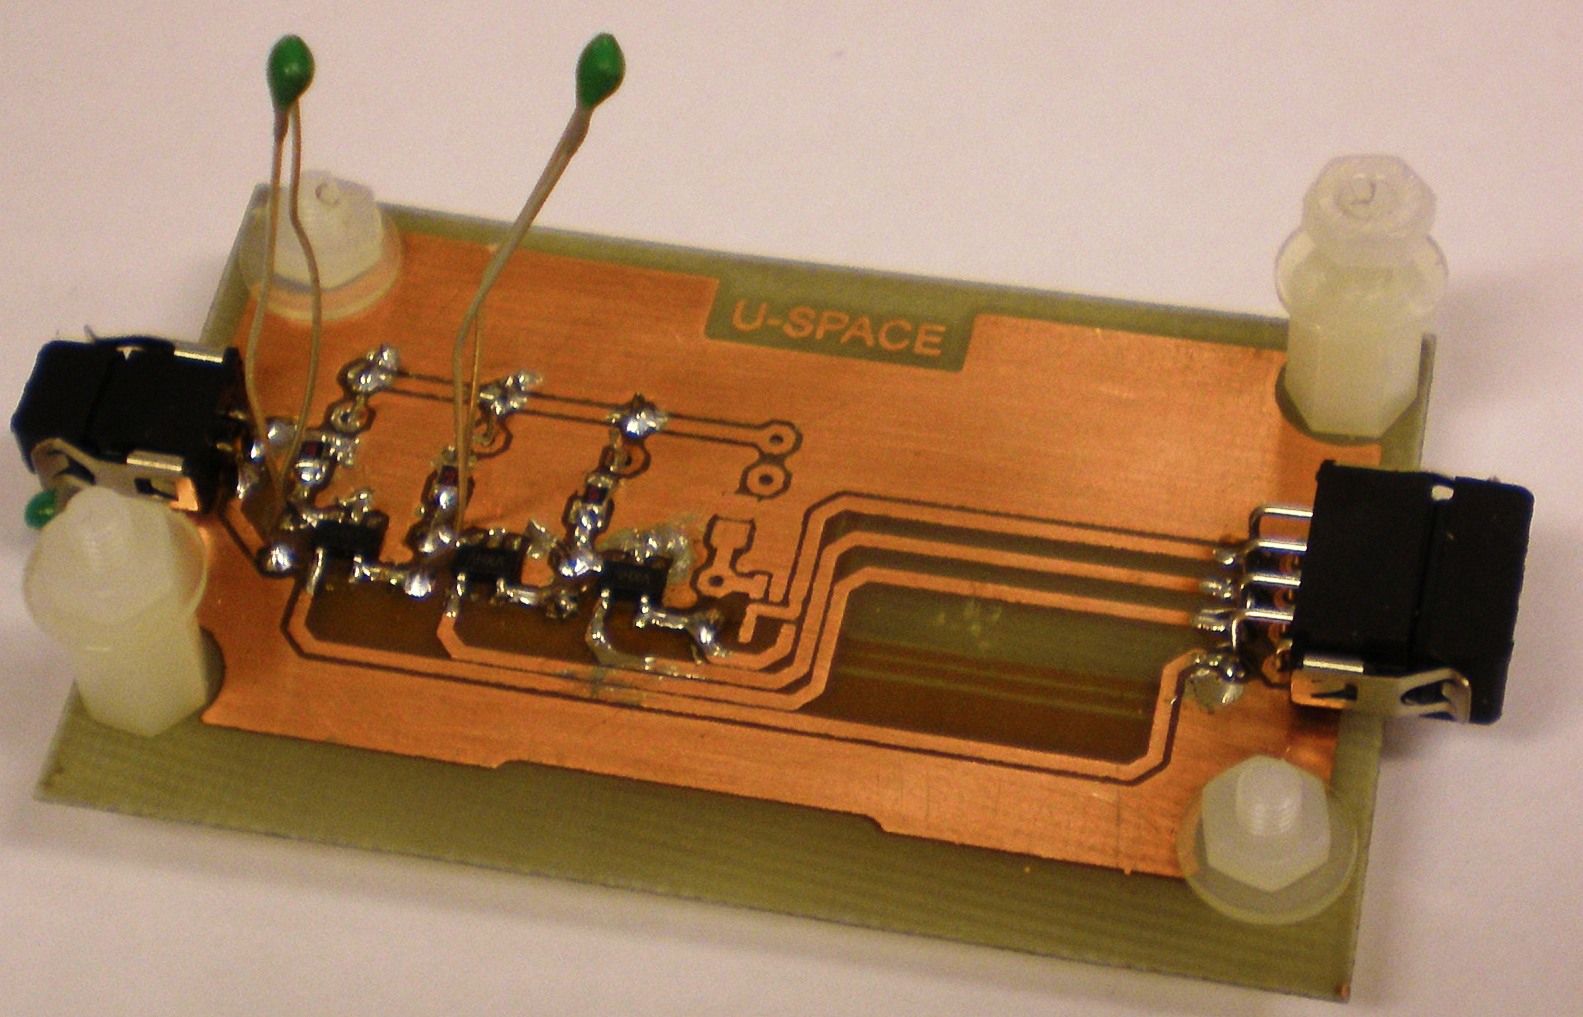
\includegraphics[width=0.7\textwidth]{figures/fig_Temp_top}
\caption{Temperature Sensor Board}
\label{fig:TS_top}
\end{figure}

\begin{figure}[H]
\centering
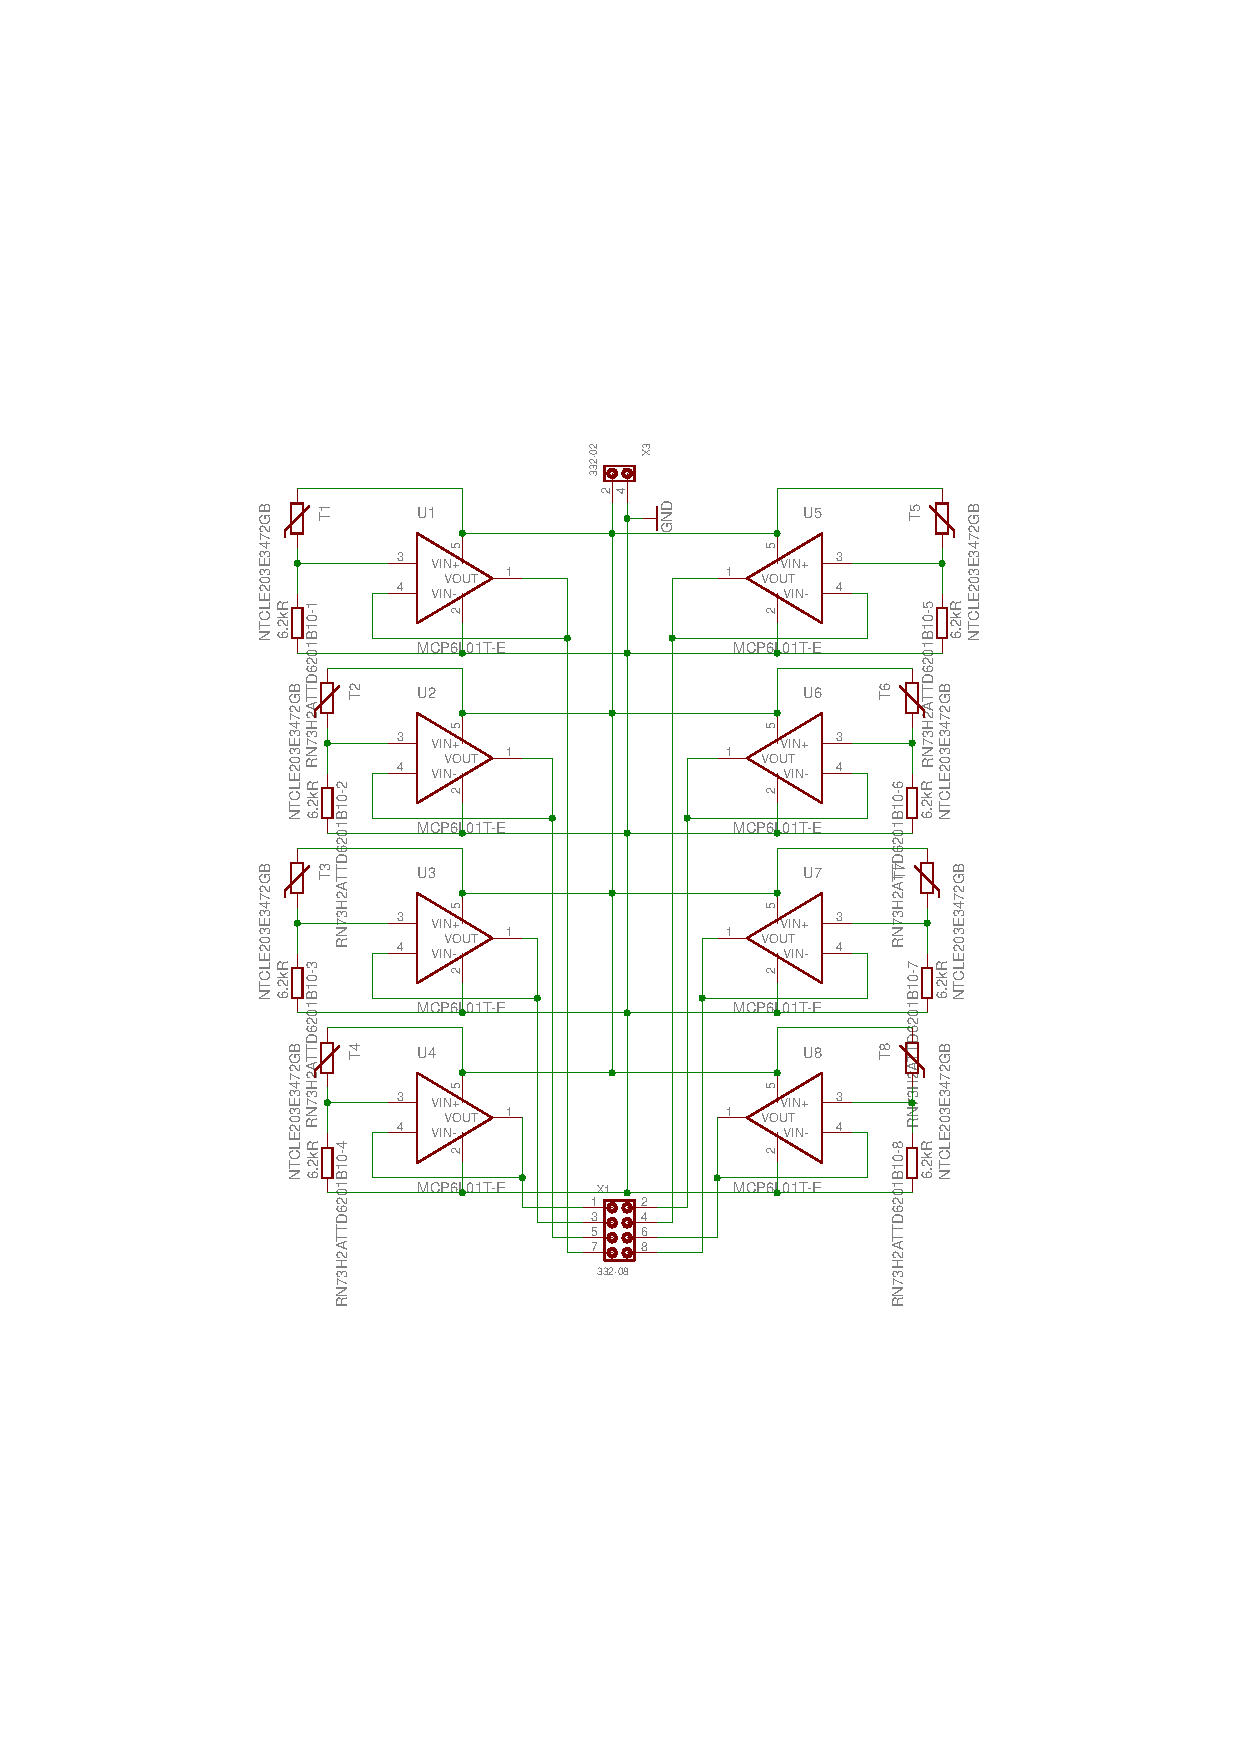
\includegraphics[width=\textwidth]{figures/fig_Schematic_TS}
\caption{Schematic of the Temperature Sensor Board}
\label{fig:Schematic_TS}
\end{figure}


\section{Mechanical Structure and Envelope}
%responsible: Pedro 

\section{Motor Control and Communication}
%responsible: Pedro and Morten

Temperature monitoring not implemented due to lack of thin wire (ordered thin wire proved to be non-practical to work with = too fragile).


\section{Imaging and Tracking Payload Unit}
%responsible: Jan

\section{Communication Subsystem}
%responsible: Omair
There is no change in the design of the \ac{TTC} subsystem from the CDR report \cite{CDR_TTC}. The \ac{U-SPACE} communication protocol was implemented in C language for the on-board computer (Beagle board) and in Lab View, due to its nice graphical environment, for the ground station. A custom \ac{PCB} was designed and developed for the conversion of analogue \acp{TM}. Second \ac{PCB} was designed for the housing and interfacing of the Xbee radio with the Beagle board. \ac{TTC} or communication subsystem provided the interface between the \ac{U-SPACE} and the ground station. This wireless connection is shown in figure \ref{fig:com_setup}. According to the test and verification plan in \cite{CDR_TTC}, testing of the on-board software and the ground station was done in Lab. However, due to one bad solder connection in the voltage level conversion board, first flight testing was not carried out.
\begin{figure}[bht]
\centering
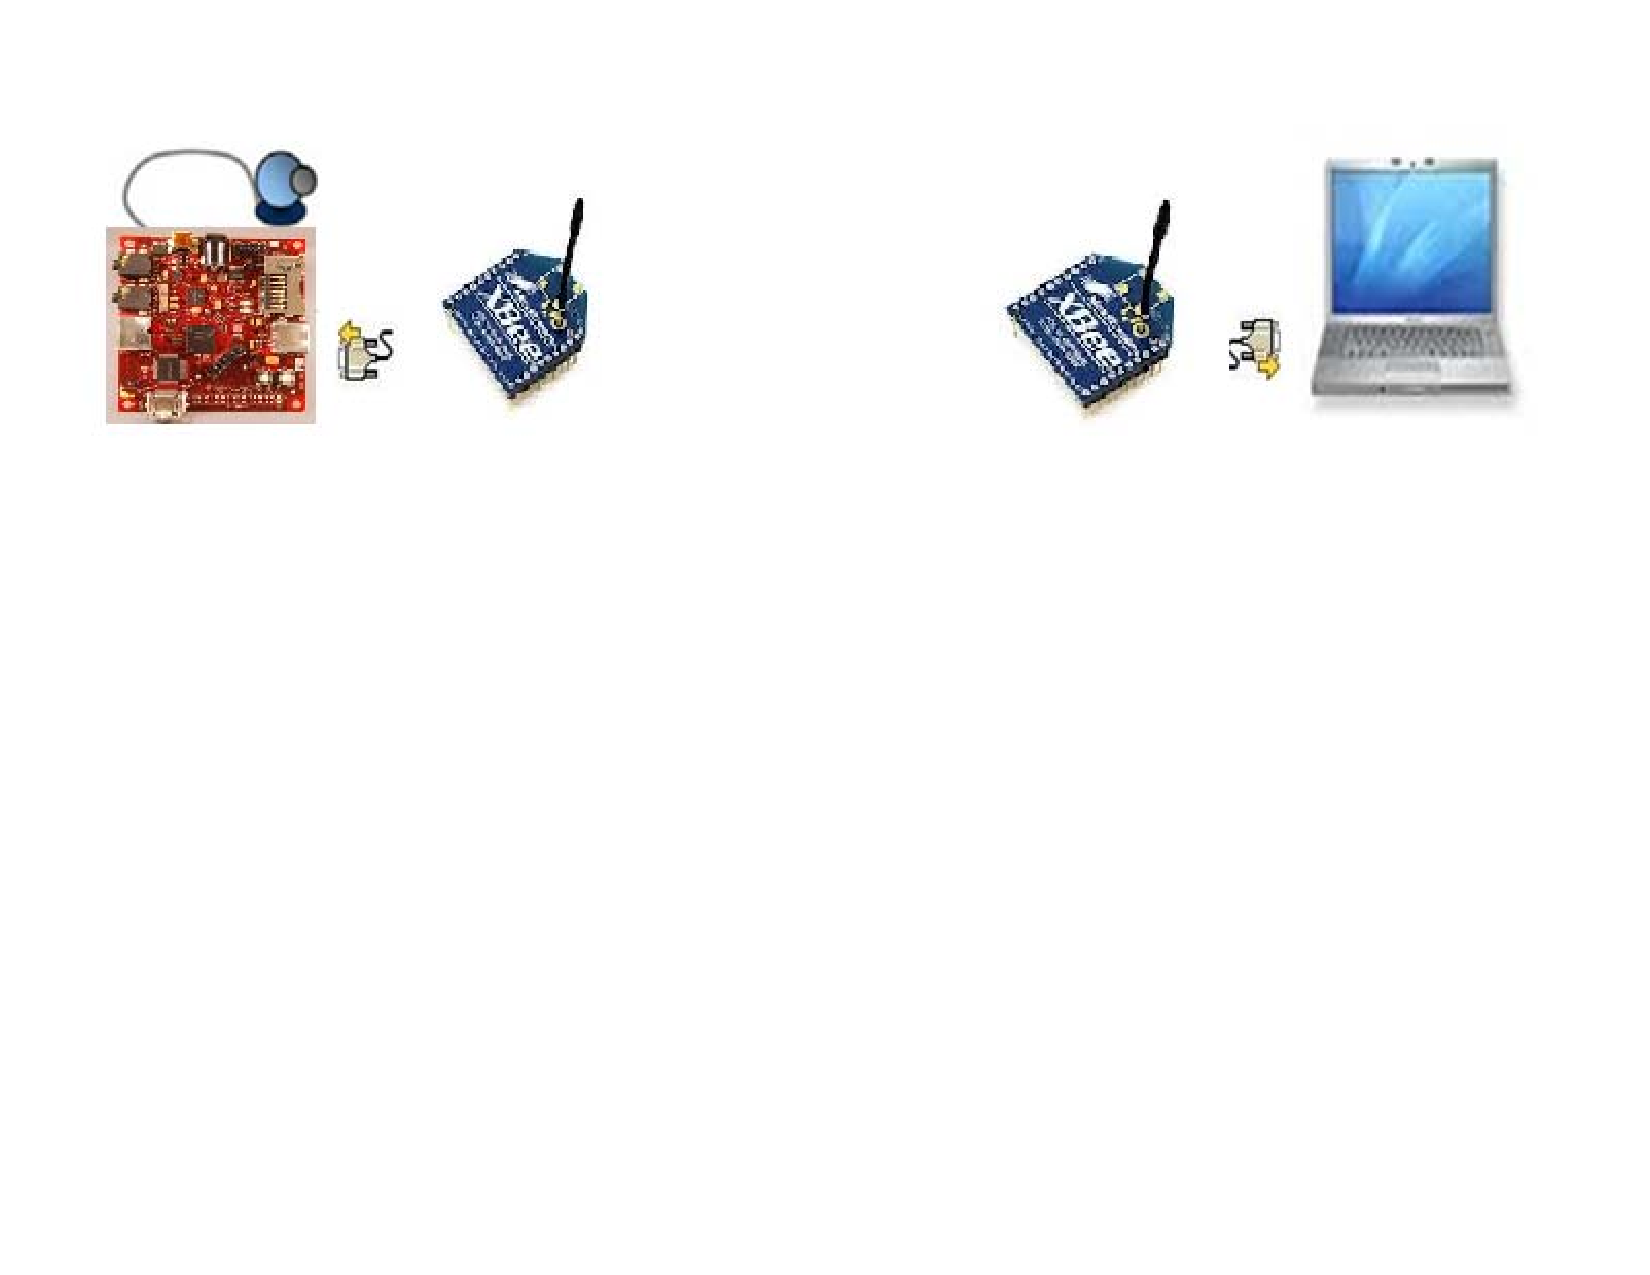
\includegraphics[scale=0.5]{figures/com_setup.pdf}
\caption[\ac{U-SPACE}Communication overview]{\ac{U-SPACE} Communication overview}
\label{fig:com_setup}
\end{figure}
%
\subsection{Telemetry}
\label{Number_of_telemetries}
In order to implement the \ac{U-SPACE} protocol, the protocol is divided into subsystems according to different functionalities; and  all the important parameters of each subsystem which need to be monitored on the ground station are considered as telemetry. Telemetry implementation details are given in table \ref{tab:telemetry_uspace}. The \ac{U-SPACE} is having a synchronization value ``$0\text{x}0C$''. Therefore for the sync field of \ac{U-SPACE} packet format, every telemetry is having a sync value of ``$0\text{x}0C$''. Power subsystem is having one byte ID $0\text{x}11$. This subsystem ID is followed by one byte parameter ID. Both subsystem ID and parameter ID makes a unique identifier TM ID within U-SPACE telemetry processing. Data size for all the power telemetries is $10$ bytes(char). \ac{OBDH} subsystem has subsystem ID of $ 0\text{x}33 $ and size of $10$ bytes for all the telemetries. The \ac{ADCS} subsystem ID is $0\text{x}55$ and it contains only one telemetry which is the attitude information of the \ac{U-SPACE}. This attitude data contains all the three rotation angles in a single packet of $30$ byte data size. The GPS subsystem ID is $ 0\text{x}77 $ and contains three telemetries; latitude, longitude and altitude of the \ac{U-SPACE}. Data size of each GPS telemetry is $10$ bytes.

\begin{table}[bht]
\centering
\caption[Telemetry list of the U-SPACE]{Telemetry list of \ac{U-SPACE}}
\label{tab:telemetry_uspace}
%\rowcolors{3}{tableshade}{white}
\begin{tabular}{|m{0.15\textwidth}m{0.1\textwidth}m{0.15\textwidth}m{0.1\textwidth}m{0.4\textwidth}|}
\hline
\textbf{Subsystem}		&  		\textbf{TM ID}				&	\textbf{size(char)}			&	\textbf{Type}& 		\textbf{Description}  			  \\ 
\hline\hline
\multirow{11}{*}{Power} &    $ 0\text{x}1141 $				&	$ 15 $						&    Analogue    &    	Under Voltage Lock-Out Status     \\
						&    $ 0\text{x}1142 $				& 	$ 15 $						& 	 Analogue	 &	 	Voltage of LiPo battery cell 2    \\
						&    $ 0\text{x}1143 $				&   $ 15 $						& 	 Analogue	 &	 	Battery discharge current  		  \\
						&    $ 0\text{x}1144 $				& 	$ 15 $						&	 Analogue	 &		Voltage of LiPo battery cell 1    \\
						&    $ 0\text{x}1145 $				& 	$ 15 $						&	 Analogue	 &		Temperature of battery  	  	  \\
						&    $ 0\text{x}1146 $				&   $ 15 $						&	 Analogue	 &		Charge controller status  	 	  \\
						&    $ 0\text{x}1147 $				&   $ 15 $						&	 Analogue	 &		Battery charge current  	  	  \\
						&    $ 0\text{x}1148 $				&   $ 15 $						&	 Analogue	 &		3.3V supply current  		 	  \\
						&    $ 0\text{x}1149 $				&   $ 15 $						&	 Analogue	 &		3.3V supply voltage  		      \\
						&    $ 0\text{x}114A $				&   $ 15 $						&	 Analogue	 &		5.0V supply current 	    	  \\
						&    $ 0\text{x}114B $				&   $ 15 $						&	 Analogue	 &		5.0V supply voltage  		 	  \\
\hline
\multirow{5}{*}{OBDH}   &    $ 0\text{x}3351 $				&	$ 15 $						&	 Analogue	 &      Temperature Motor 1			      \\
						&    $ 0\text{x}3352 $				&	$ 15 $						&	 Analogue	 &      Temperature Motor 2	   		      \\
						&    $ 0\text{x}3353 $				&	$ 15 $						&	 Analogue	 &      Temperature Atmosphere		      \\
						&    $ 0\text{x}3354 $				&	$ 15 $						&	 Analogue	 &      Temperature Electronics Bay	      \\
						&	 $ 0\text{x}3355 $				&	$ 35 $						&	 Digital	 &      UTC Time					      \\
\hline
\multirow{1}{*}{ADCS}   &    $ 0\text{x}5561 $ 				&	$ 35 $						&	 Digital	 &	    Roll, Yaw and Pitch	       		  \\
\hline
\multirow{3}{*}{GPS}    &    $ 0\text{x}7771 $				&	$ 15 $						&	 Digital	 &      Latitude		       	    	  \\
						&    $ 0\text{x}7772 $				&	$ 15 $						&	 Digital	 &      Longitude	   				      \\
						&    $ 0\text{x}7773 $				&	$ 15 $						&    Digital	 &      Altitude  				          \\ 
\hline
\end{tabular}
\end{table}
%

\subsection{Telecommands}
\label{subsec:telecommand}
Table \ref{tab:telecommand_uspace} gives the list of implemented telecommands for the \ac{U-SPACE}. Telecommands can be sent to configure the on board computer for different modes of telemetry or configure a specific subsystem. There are six different modes of the telemetry which are listed in table \ref{tab:TM_modes} along with the data rate for each mode. These modes can be configured by sending telecommands. All these telecommands are implemented under the \ac{OBDH} subsystem. Details of implementation according to the telecommad format are given in table \ref{tab:telecommand_uspace}.
%
\begin{table}[bht]
\centering
\caption[Data rate for different \ac{TM} modes]{Data rate for different \ac{TM} modes}
\label{tab:TM_modes}
%\rowcolors{3}{tableshade}{white}
\begin{tabular}{|m{0.4\textwidth}m{0.4\textwidth}|}
\hline
\textbf{TM mode}			&  		\textbf{Data rate(bps)}   \\
\hline
Switch off telemetries		&		$ 0 $		 			  \\
Power only	   		        &		$ 1320 $		 		  \\
\ac{OBDH} only	      	  	&		$ 760 $		 			  \\
ADCS only			      	&		$ 280 $		 			  \\
GPS only		   		    & 		$ 360 $		 			  \\
All telemetries	      	  	&		$ 2720 $		 		  \\
\hline
\end{tabular}
\end{table}
Three telecommands are implemented for the payload (camera). Camera set command is implemented to set the time interval between two successive images. After setting the image interval, camera start command is used to instruct the on-board computer to take picture after the specified time interval. Third is the camera stop command which will stop the camera. In future, if some one implements the real time pulse width modulator using a micro controller or beagle board, commands for speed control of the motor can be incorporated. Then, the use of joystick can be discarded and U-SPACE will be fully controlled by the Xbee radio link only.

\begin{table}[bht]
\centering
\caption[Telecommand list of the U-SPACE]{Telecommands of \ac{U-SPACE}}
\label{tab:telecommand_uspace}
%\rowcolors{3}{tableshade}{white}
\begin{tabular}{|m{0.15\textwidth}m{0.1\textwidth}m{0.15\textwidth}m{0.2\textwidth}m{0.25\textwidth}|}
\hline
\textbf{Subsystem}		&  		\textbf{TM ID}				&	\textbf{size(char)}		&	\textbf{Data field}	& 		\textbf{Description}  	  \\ 
\hline\hline
\multirow{9}{*}{OBDH}   &    $ 0\text{x}33B2 $				&	$ 16 $					&	image interval		&      Camera Set			      \\
						&    $ 0\text{x}33B3 $				&	$ 16 $					&	$ 0\text{x}00 $		&      Camera Start	   		      \\
						&    $ 0\text{x}33B4 $				&	$ 16 $					&	$ 0\text{x}00 $		&      Camera Stop		      	  \\
						&    $ 0\text{x}33B1 $				&	$ 16 $					&	$ 0\text{x}00 $		&      Switch off telemetries	  \\
						&    $ 0\text{x}33B1 $				&	$ 16 $					&	$ 0\text{x}10 $		&      Power only	   		      \\
						&    $ 0\text{x}33B1 $				&	$ 16 $					&	$ 0\text{x}20 $		&      \ac{OBDH} only	      	  \\
						&    $ 0\text{x}33B1 $				&	$ 16 $					&	$ 0\text{x}40 $		&      ADCS only			      \\
						&    $ 0\text{x}33B1 $				&	$ 16 $					&	$ 0\text{x}50 $		&      GPS only		   		      \\
						&    $ 0\text{x}33B1 $				&	$ 16 $					&	$ 0\text{x}70 $		&      All telemetries	      	  \\
\hline
\end{tabular}
\end{table}
\subsection{Telemetry Conversion Module}
Type of the telemetry in table \ref{tab:telemetry_uspace} is stated analogue if the sensor does not have a built in \ac{ADC} and requires an external \ac{ADC} for its on board processing. Also, the Beagle board does not have \ac{ADC} chip on board. So a custom \ac{PCB} shown in figure \ref{fig:PCB_conversion_module} has been designed, etched and soldered in the lab which is capable of converting all the analogue telemetries listed in table \ref{tab:telemetry_uspace} into digital domain. In the design of the conversion module, two ADC chips (ad7998) are used from analog devices. AD7998 is a 12 bit \ac{ADC} chip having eight input channels and a multiplexer on a single IC. For the protection of the IC from high input voltage, diodes are added. These diodes get forward biased, if the telemetry voltage goes above $5$V, connecting the input pin to the power supply of the IC.  A second PCB has been designed for the housing of on-board X-bee pro module. This \ac{PCB} will be used to interface the Xbee pro module to the beagle board for transmission and reception of the telecommands and telemetries respectively.\\
%
\begin{figure}[bht]
\centering
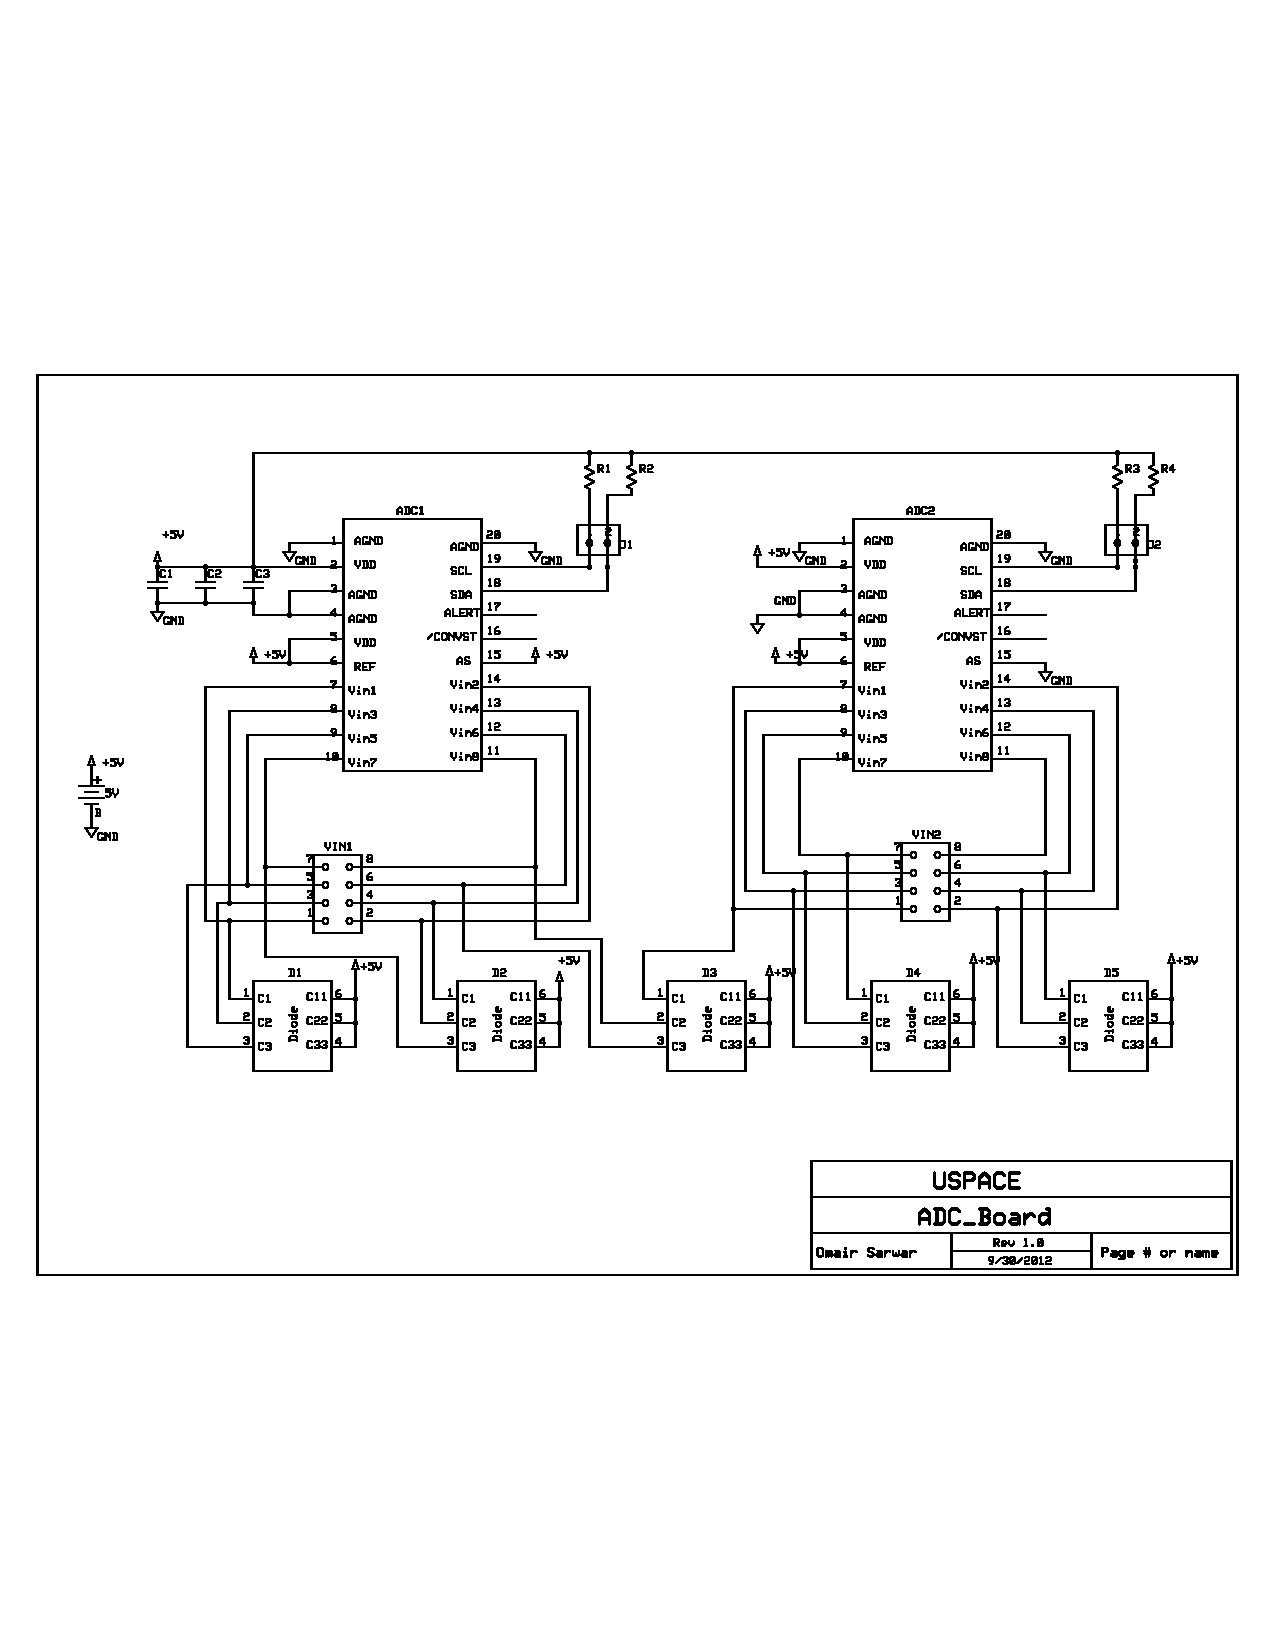
\includegraphics[scale=0.7]{figures/schematic_conversion_module.pdf}
\caption{Schematic of telemetry conversion module}
\label{fig:schematic_conversion_module}
\end{figure}

\begin{figure}[bht]
\centering
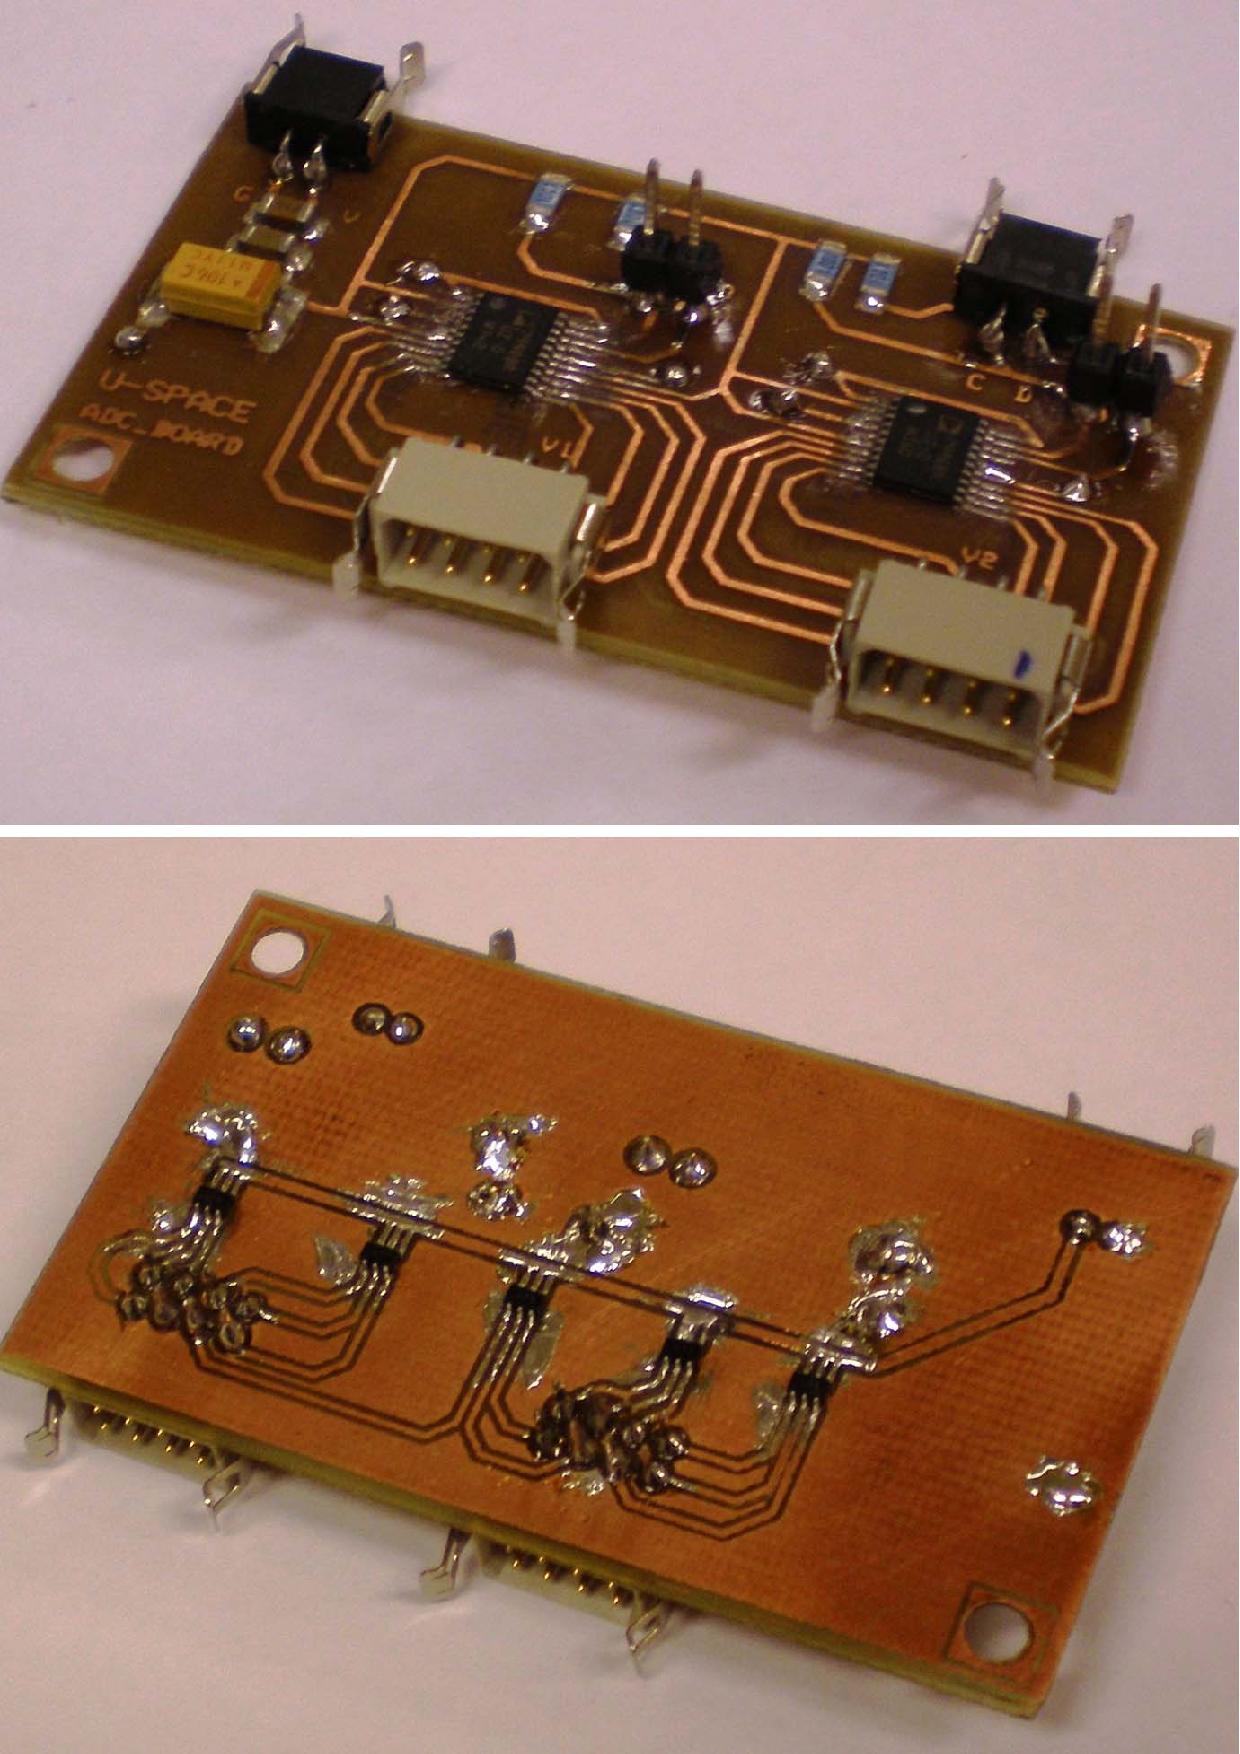
\includegraphics[scale=0.45]{figures/PCB_conversion_module.pdf}
\caption{\ac{PCB} of Conversion module}
\label{fig:PCB_conversion_module}
\end{figure}
%
Interfacing of the conversion module with the beagle board is shown in figure \ref{fig:conversion_module}. AD7998 gives the data along with the channel ID on I$2$C bus of $5$V. Beagle board has an I$2$C bus and the conversion board can be easily integrated to it. However, the I$2$C interface of the Beagle board is at a voltage level of $1.8$V so that a voltage conversion board (level converter) has been developed (refer \cite{CDR}) for the conversion of $5.0$V and $3.3$V I$2$C bus to $1.8$V I$2$C bus.
%
\begin{figure}[bht]
\centering
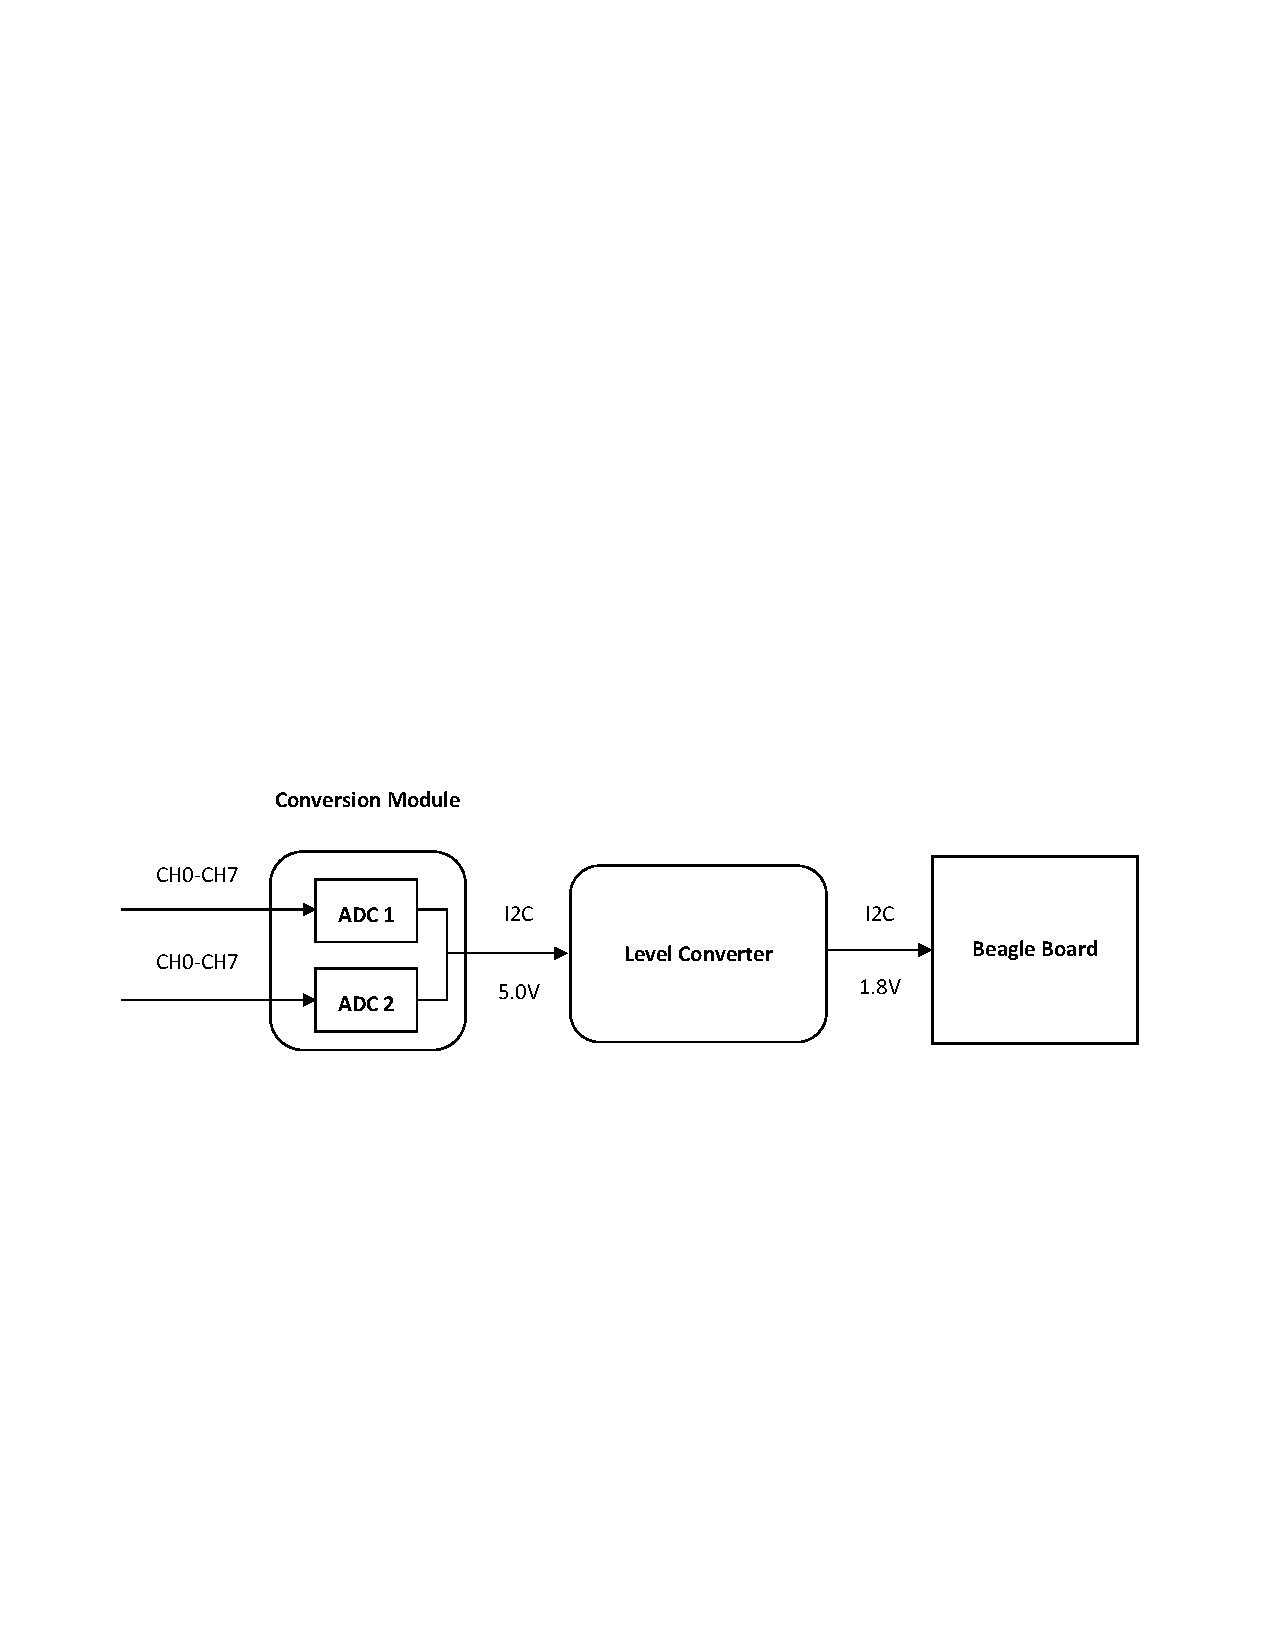
\includegraphics[scale=0.7]{figures/conversion_module.pdf}
\caption{Conversion module interface with Beagle board}
\label{fig:conversion_module}
\end{figure}
\subsection{U-SPACE Ground Station}
Programming language for the ground station was Lab View software. The front panel view of the \ac{U-SPACE} ground station is shown in figure \ref{fig:Labview_ground_station}. Here, I will discuss how to use \ac{U-SPACE} ground station. There is serial communication between the computer running the ground station software and the Xbee radio. To configure parameters for this communication, there is one section ''COM'' in the ground station. Here, we can set data rate, parity bit, start and stop bit. These parameters should be the same as configured for the on-board computer. There is also a ``Debug'' window which displays the serial communication data for debugging purposes. \\
%
For generating the telecommands, there is one section on the upper left part of the front panel of the ground station. First of all, select the subsystem to which you to want to send the telecommand. This will cause the subsystem to select subsystem ID in the background. Then select the property (parameter) you want to configure. This will cause the selection of property ID of the subsystem. Finally fill data field with the appropriate value in accordance to on-board computer software. On clicking the ``SEND'' button, it will generate the telecommand and send it through the Xbee radio. Concatenated telecommand according to \ac{U-SPACE} communication format can be shown in ``Debug'' window. A separate telecommand section is also dedicated to configure the \ac{U-SPACE} telemtry modes as described in section \ref{subsec:telecommand}. Select the mode from the drop down menu and click ``SEND TM'' button.
\\
  %
\begin{figure}[bht]
\centering
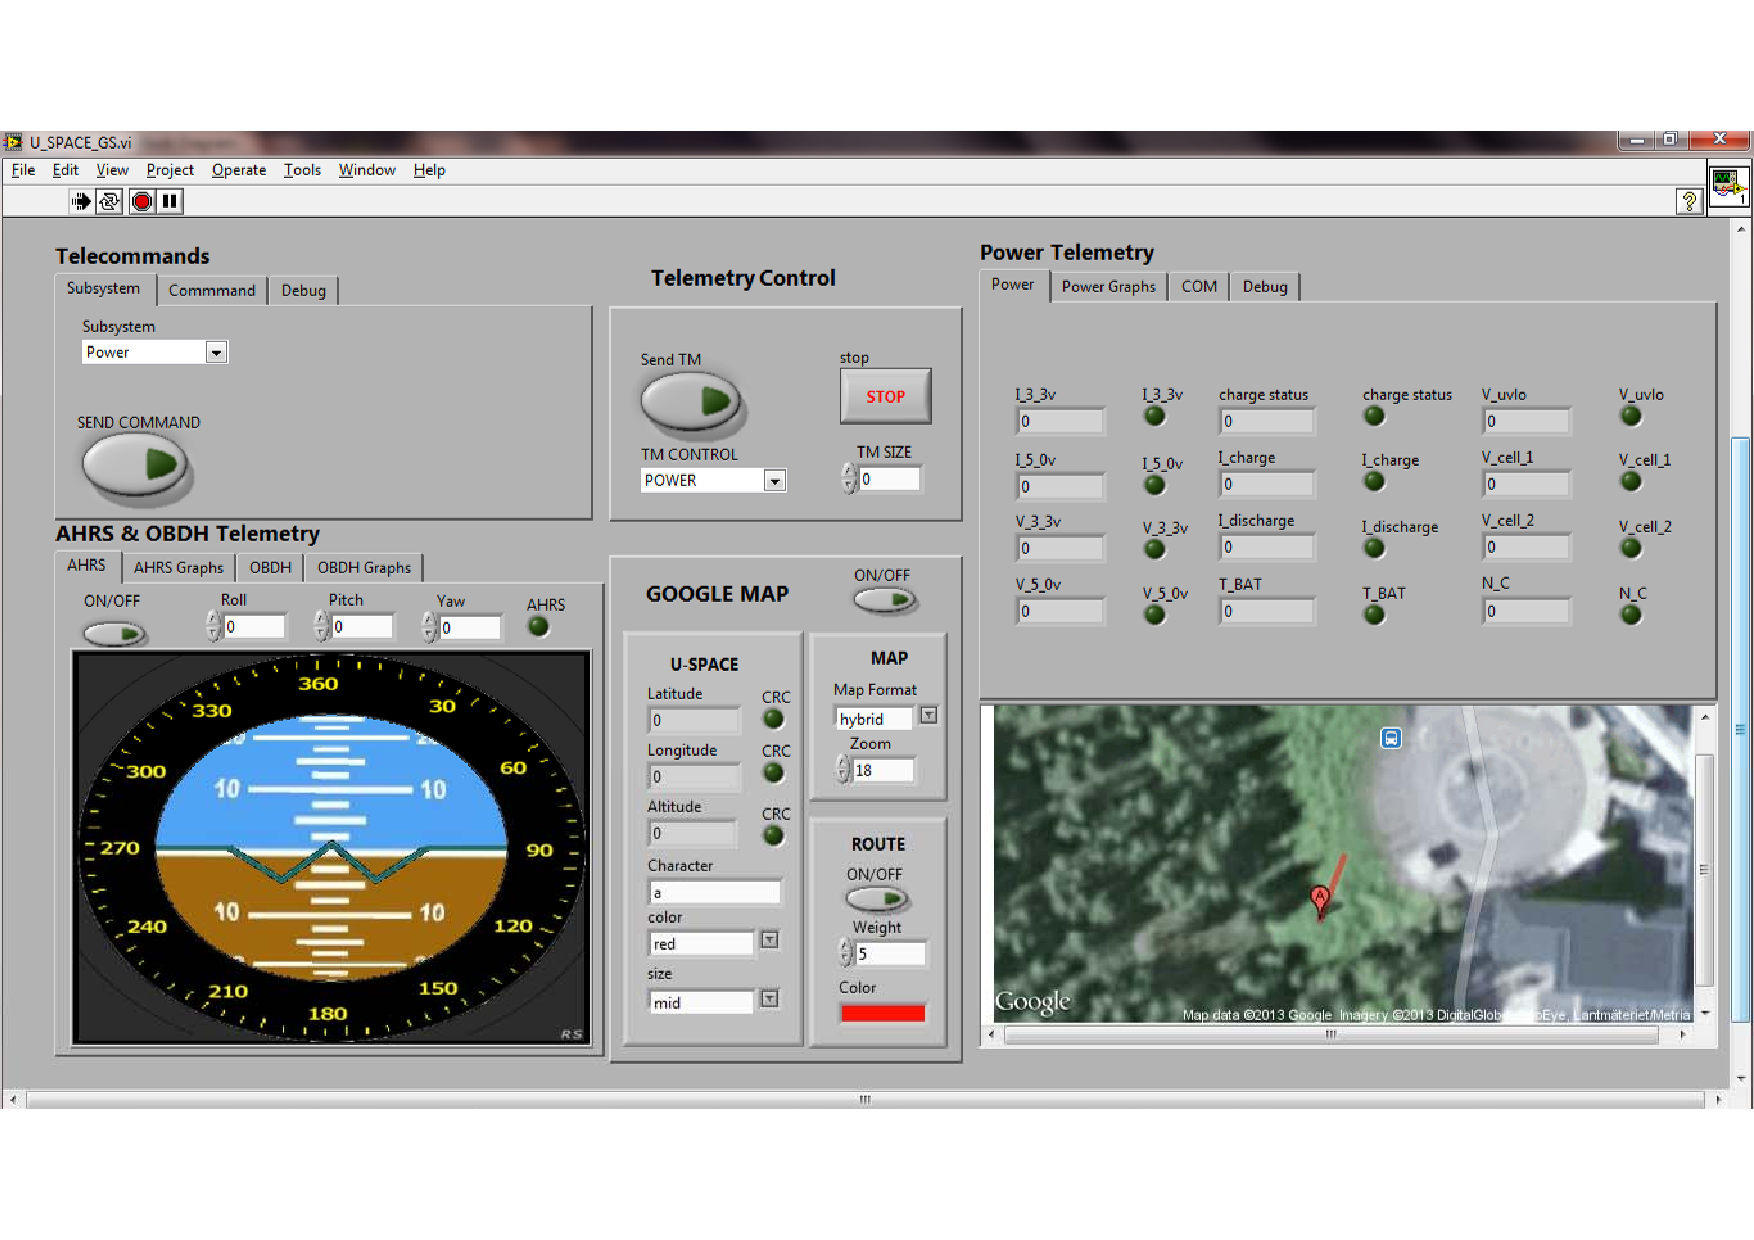
\includegraphics[scale=0.5]{figures/GS.pdf}
\caption{U-SPACE ground station Lab View Front Panel}
\label{fig:Labview_ground_station}
\end{figure}
%
On the front panel of the ground station, telemetries are displayed in groups according to the subsystem. Power telemetries are on the upper right corner. All the eleven telemetries are shown in numerical display. There are three telemetries in the power graphical display; battery voltage, battery current and discharge current. To see the graphical display, go to ``Power graphs'' and then select the telemetry for graphical display from drop down menu.\\ 
\ac{ADCS} and \ac{OBDH} telemetries are shown in left lower corner. \ac{ADCS} contains three attitude parametrs; roll, pitch and yaw in numerical display. If you want, these to be displayed on the artificial horizon, click the ON/OFF button. Artificial horizon consists of three images: first, for roll; second for pitch; third for heading and moves them relatively according to the input attitude data. All the \ac{OBDH} telemetries are displayed numerically in a separate window which is embedded with the \ac{ADCS} subsystem. However four \ac{OBDH} temperatures: ambient, cargo bay and one of each motor are also displayed in the ``\ac{OBDH} graph window'' Here you can see the rate of change of temperature during different phases of flight of the \ac{U-SPACE}. \\
For the GPS subsystem, telemetries are shown in numerically in the right lower corner of the front panel view of the ground station. To show the position of the \ac{U-SPACE} on google maps, an internet connection is required. This is a static image implementation of the desired lattitue, longitude, image size and the resolution. Select the \ac{U-SPACE} indicator parameters: character (showing \ac{U-SPACE}), colour and font for display. Also select the type of map and click the google maps ``ON/OFF'' button. This will generate a \ac{URL} according to the selected characteristics and will download the corresponding static image from google maps. To show the route of the \ac{U-SPACE} from starting point, select route characteristics and click show route ``ON/OFF button''. This will track the \ac{U-SPACE} from the starting point.
